\documentclass[a4paper, 10pt, english, final]{report}
%\usepackage[utf8]{inputenc}
%\usepackage{a4wide}

\usepackage[draft]{fixme}



%%%%% TYPE SETTING %%%%%
\usepackage[T1]{fontenc}
%\usepackage{garamond}
%\renewcommand{\rmdefault}{ugm}

\usepackage[british]{babel}
\usepackage{verbatim}

\usepackage{palatino}              % font : garamond
\linespread{1.05}                  % Palatino needs more leading (space between lines)
\renewcommand{\ttdefault}{cmtt}    % alternative monospace font

%%%% MATH STUFF %%%%%%
\usepackage{amsmath}
\usepackage{amssymb}
\usepackage{ulem}
\usepackage{mathrsfs}

%%%% GRAPHICS
\usepackage{graphicx}
\usepackage{hyperref}
\usepackage{listings}

\usepackage{float}
\usepackage[small,bf]{caption}
%\usepackage{xypic}
\usepackage[table]{xcolor}
\usepackage{subfig}
%\usepackage{dirtree}
\usepackage{ulem}
\usepackage{slashbox}

%%%%%%%%%%%%%%%%%%%%%%%%%%%%%%%%%%%%%%%%%%%%%%%%%%%%
%%%%% CONFIGURATIONS %%%%%%
%%%%%%%%%%%%%%%%%%%%%%%%%%%%%%%%%%%%%%%%%%%%%%%%%%%%
\lstset{language=Python, basicstyle=\scriptsize, showstringspaces=false, numbers=none, stepnumber=1, numberstyle=\tiny}

\hyphenation{mand-en} %%% Add here if something does not break right. Like this nu-clear-test-bomb-ing


%%%%%%%%%%%%%%%%%%%%%%%%%%%%%%%%%%%%%%%%%%%%%%%%%%%%%%%%%%%%%%%%
% Kommandoer
%%%%%%%%%%%%%%%%%%%%%%%%%%%%%%%%%%%%%%%%%%%%%%%%%%%%%%%%%%%%%%%%
%\newcommand{\old}[1]{\oldstylenums{#1}}
%\newcommand{\old}[1]{{#1}}
\newcommand{\mailto}[1]{\href{mailto:#1}{#1}}
%\newcommand{\resume}[1]{\begin{abstract}{\sffamily #1}\end{abstract}}
%\newcommand{\angles}[1]{\langle\textrm{#1}\rangle}
%\newcommand{\colbox}[2]{\fcolorbox{black}{#1}{#2}}
%\renewcommand{\thefigure}{\thechapter.\thesection.\arabic{figure}}
%\renewcommand{\thetable}{\thechapter.\thesection.\arabic{table}}

%%%%%%%%%%%%%%%%%%%%%%%%%%%%%%%%%%%%%%%%%%%%%%%%%%%%%%%%%%%%%%%
% Titel, forfatter og dato
%%%%%%%%%%%%%%%%%%%%%%%%%%%%%%%%%%%%%%%%%%%%%%%%%%%%%%%%%%%%%%%

\title{Support decision system for diagnosing rare diseases using machine learning for medical text mining}

\author{Henrik G. Jensen - \mailto{henrikgjensen@gmail.com} \and
  Michael Andersen - \mailto{michael.blackplague.andersen@gmail.com} \\
\\
Project supervisor \\ 
Ole Winther - \mailto{owi@imm.dtu.dk} \\
\\
Co-supervisor \\ Henrik L. J\o rgensen - \mailto{hlj@dadlnet.dk}}

\date{\today}

\hypersetup{
colorlinks,%
citecolor=black,%
filecolor=black,%
linkcolor=black,%
urlcolor=black,%
bookmarksopen=false,
pdftitle={Support decision system for diagnosing rare diseases using machine learning for medical text mining},
pdfauthor={Henrik G. Jensen and Michael Andersen},
pdfsubject={Text mining, rare diseases},
pdfkeywords={Diagnosing rare diseases, text mining}
}

%%%%%%%%%%%%%%%%%%%%%%%%%%%%%%%%%%%%%%%%%%%%%%%%%%%%%%%%%%%%%%
% Indhold
%%%%%%%%%%%%%%%%%%%%%%%%%%%%%%%%%%%%%%%%%%%%%%%%%%%%%%%%%%%%%%
\begin{document}
\maketitle
\pagenumbering{roman}
\thispagestyle{empty}

\abstract
It can be time consuming for a physician to diagnose a disease and
even more so if it is a rare disease. Many rare disease have a high
fatality rate so a quick diagnosis is vital to the health of the
patient. We therefore propose a prototype support decision system for
diagnosing rare diseases with a specialized database. For this we will
be using a vector space model to look for similarity between input
symptoms and gathered information. Given a list of symptoms, the
system will calculate a similarity score between the search query and
the documents in the matrix. The system was tested using 13 test cases
from BMJ \cite{HangwiTang11102006}, 29 test cases from Orpha.net and 5
blind tests cases provided by chief physician Henrik J\o rgensen and
Lennart Friis-Hansen. In a top 20 the system returned the correct
results for 8 out of 13 for BMJ, 20 out of 29 for Orpha.net and 3 out
of 5 during the blind test. The system places $61.5\%$ of the BMJ
cases, $68\%$ of Orpha.net and $60\%$ of the blind test cases in top
20. This proves the potential of the system, and suggests that further
work within this area of research should be performed.


\addcontentsline{toc}{chapter}{Acknowledgements}
\chapter*{Acknowledgements}
We would like to thank our supervisor for letting us take on this
project, even though the project was not clearly defined from the
beginning. His ideas and thoughts helped us a lot when we ran into
corners.

We would like to thanks Henrik L. J\o rgensen for supplying blind test
cases on which to perform tests. And for his input to the project in
general.

We would like to thank Lennart Friis-Hansen for coming up with the
original idea for the project, and hope that others --- in the future
--- will continue our project, or others similar to it.

We would also like to thank the IT-department at the Institute of
Computer Science at Copenhagen University for allowing us to use one
of their machine for our data/text processing, without it this project
would never have been possible.

We would also like to thank the Institute of Computer Science for
allowing 24/7 access and the cantina, for coffee and facilities for
making edible meals.

And last but not least we would like to thank our friends and loved
ones for support during, especially the last three weeks of the
project.


\tableofcontents

\chapter{Introduction\label{Introduction}}

Due to the vast amount of information available on the Internet today,
it is near impossible for researchers to have an 'up-to-date'
knowledge on everything but their own specific field. Even that seems
to become more and more difficult as new information is added each
day\footnote{Take for instance the biomedical database MedLine that
  grows with over half a million citations per year}
\cite{CitAddMedLine}. Therefore it can be necessary to employ tools to
help gather, structure and look for relations or hypothesis within the
piles information. One very popular method of finding new relations in
data is through the use of \textit{text mining}.

\begin{center}
{\small``The whole is greater than the sum of its parts'' $\sim$ Aristotle
(384--322 BC)} 
\end{center}

Text mining refers to the automated search for meaningful patterns in
structured or unstructured text documents stored in very large digital
databases or distributed over the Web. A good example of this is
``Fish oil, Raynaud's syndrome and undiscovered public knowledge'' by
D.R. Swanson \cite{DRSwanson}. Here Swanson was referring to published
knowledge deeply buried in disjoint topical domains\footnote{Here
  'disjoint' refers to articles written by researchers unaware of each
  others work}. Swanson was one of the first to propose using text
mining on biomedical literature. In 1986, he found evidence of a
relation between the use of fish oil and the development of Raynaud's
syndrome by looking at seemingly unrelated documents. This was done
years before there were actually any scientific documents supporting
this.

Over the recent years the use of text mining has grown
tremendously. In the biomedical field, research is divided into highly
specialized sections and subsections often too complex to make room
for interdisciplinary work. For instance, the recent sequencing of the
human genome have introduced a whole new level of detail to genetic
research. It is likely that new discoveries in this area could affect
other areas concerned with health and diseases since genomic
mechanisms play a major role in the various branches of medicine
\cite{survey.biomed.text.cohen.2005}. Text mining is a way of making
these important connections in a world of increasing complexity and
hidden patterns. This way of making new unseen discoveries also
introduces text mining as a major potential aid in the diagnosis of
rare or (to the physician) unknown diseases.

This project aims to make it easier and more efficient for physicians
in diagnosing rare diseases. Through the use of text mining,
clustering and machine learning algorithms, it is an attempt to
increase the likelihood of getting the correct article based on a
search of symptoms, environmental and/or human factors. We use a list
of rare diseases and synonyms acquired from Rarediseases.info
\cite{Rarediseases}. Based on this, we
extract a series of MedLine records \cite{PubMedFactSheetMedline}
using the Python module Bio.Entrez \cite{EntrezProgUtil} and process
the text for a more optimized search.

\section{Inspiration}

The list of rare diseases counts over 6,000 and has 5
added to it a week \cite{AboutRareDiseasesOrphanet}. A rare (or
orphan) disease is classified by the Orpha.net Encyclopedia
\cite{OrphanetEncyclopedia} as being a disease that affects less than
1 out of 2,000 people in Europe and has severe chronic or terminal
outcomes (or less than 200,000 affected in the USA by standard of
Rarediseases.info \cite{Rarediseases}). Some of these \fxnote{fix -
  some of these diseases} diseases might not be fatal if treated in
time. However, given the amount of knowledge your physician would need
to carry around to make a correct diagnosis (or correctly exclude
other potentials), a quick (and correct) treatment is not always the
case.

When being affected by a rare disease, the lack of a correct diagnosis
--- or the delay spent going from one specialist to another --- will in
often lead to a fatal outcome. When it comes to rare and often
dangerous diseases, the typical physician has little or none prior
experience with similar cases. Therefore it is important that the
diagnosing physician has as much help at hand as possible in this
intrinsic task.

In a dialogue with Henrik L. J\o rgensen \cite{TheDude} --- chief
physician at Bispebjerg Hospital --- we found that --- even though
many systems already exist to help physicians in their diagnosis ---
there seemed to be a lack of a system for specifically diagnosing rare
diseases. Systems such as PubMed returns numerous results if the
symptoms are slightly non-specific (more on this in the following
chapters). The advantage of a specialized system for rare diseases
would be that the physician --- being in doubt --- would have a chance
to make a quick symptom look-up before referring or dismissing the
patient. According to Henrik L. J\o rgensen, time is great a problem
when treating patients and in the rare event of a patient being
affected by something unknown, he or she is referred to a specialist.

The inspiration of being able to create an efficient support decision
system for diagnosing rare diseases was what drove us to initiate this
project.

\section{Objectives}

\subsubsection{Aim}
Our system will be based on machine learning concepts and will
hopefully add something new to the arena of medical support decision
systems. Testing various techniques to optimize our system, we aim to
design a system that --- if successful --- also has the generic potential of
being expanded to other domains than that of rare diseases.

\subsubsection{Overall process}
The list of rare disease names (along with synonyms and optional
descriptions) will be mined from the Rarediseases.info website. Some
of these diseases will have specialized PubMed search strings that we
mine along with the names. Using these names, predefined search
strings and synonyms, we search PubMed for a maximum of 500
PMID's\footnote{PMID's are unique article identifiers used by PubMed}
per disease, representing MedLine records containing an abstract. We
then download the corresponding records.

The intention is to preprocess the data using a vector space model and
various heuristics to optimize the probability of getting a correct
hit. The heuristics are described in the following chapter but
revolves mainly around the Term Frequency - Inverse Document Frequency
(TF-IDF). Since a graphical user interface will not be made for the
prototype system, a correct hit is as an article defining the disease
being among the top 20 returned results from a given query of
symptoms.

We will be running tests on three different test cases. The first set
of cases are derived from a subset of tests in the BMJ article
\cite{HangwiTang11102006} relevant to our database\footnote{We only
  run tests on the diseases present in our database} The second set of
cases come from a random select of disease descriptions on the
Orpha.net website \cite{Orphanet}. The third and final set of test
cases come from a blind test provided by Henrik L. J\o rgensen.

\fxnote{tilfoej lennart hvis han kommer med noget}

\subsubsection{Primary tools}
We will be using Python 2.6.2 \cite{PythonLanguage} in this project. For access to PubMed, we use
the Python module Bio.Entrez \cite{EntrezProgUtil} while BeautifulSoup
\cite{BS} is used for parsing of HTML/XML combined with Urllib2
\cite{UL2} these are used for crawling the websites. For construction
of the term document matrix, we use the SciPy package \cite{SciPy}
which supports sparse matrix structures. And for auxiliary vector
functions we use the Numpy package \cite{NumPy}.

\section{Roadmap}

Chapter \ref{Background} covers the different databases that we
harvest our data from and how we intend to model it the
information. We provides a background on Rarediseases.info, PubMed and
the MedLine database, our primary data sources. We examine various
advantages and disadvantages of the models and heuristics that we use,
how we measure the similarities used to provide a disease score for
queries, we also look into the data types used to handle the large
amounts of information. Lastly, we looks at an alternative that might
be able to provide more information on each mined disease.

Chapter \ref{Methods} deals with the methods that we have used to
implement the first prototype and the following branches of the
system. We give an overview of the implementation and we increase the
flexibility of the data exchange between the modules and how we have
applied several heuristics/filters to the data and the vector
space. The chapter is \fxnote{The chapter is rounded of...} rounded of
with details of the data and technical conclusions of the
implementation.

Chapter \ref{ExperimentsResults} contains all the primary tests and
results of the different schemes used to find the most efficient model
for looking up rare diseases. The cosine similarity measure and the
simple sum similarity measure are tested, measured and put up against
each other to see which performs the best. This is done on both the
classical term document matrix and on a document-summed version called
the \textit{disease matrix}. It also deals with aspects and tests of
clustering and some of the potential noise in the data set.

Chapter \ref{Conclusion} is the conclusion of the project. It contains
a summary of the results along with comments on the usefulness of
a system from by Henrik L. J\o rgensen.


Chapter \ref{FutureWorks} contains future perspectives of the project,
what could it become and which features could be useful if the system
were to be made available for use by physicians all over the world.



\chapter{Background\label{Background}}

This chapter examines the advantages and disadvantages of diagnosing
rare diseases, of the places we harvest data from and of the data
models we intend to use, including applied heuristics for
optimization. We will reason our choices through the preliminary work
of others and look at alternatives to the some of the choices made. We
will also go through many of the theoretical aspects of the methods
used for the prototype system.\\

We start by looking at some of the difficulties that follow with
diagnosing rare diseases and how we approach the problem. Following
this, we give an introduction to the Rarediseases.info website and to
the structure of PubMed and the subset of PubMed that we use -
MedLine. We will be looking at how these websites and databases can be
used for our prototype system. We then move on to the advantages and
disadvantages of the vector space model that represents one of the
most common ways to structure document data. We look at heuristics
that can be applied before and on the vector space model to optimize
the way the document data is represented in relation to one
another. We also go through the most commonly used vector similarity
measure, the cosine measure, and mention another simpler scoring
measure that we intend to use for scoring queries. Finally we give a
short describtion of the data structures we intend to use for storing
data, and we look into mention worthy alternative to Rarediseases.info
when it comes to information on rare diseases.

\section{Diagnosing rare diseases}

In theory, clinical decision-making is a complicated process based on
experience, judgement and a reasoning coming from a large integrate of
medical literature and clinical trials. In practise though, a
physician may have very little time per patient and, when in doubt,
must come with a qualified guess based on personal experience and
judgement. But with the tremendous knowledge available today, the
physician should not stand alone with this decision-making. If the
symptoms of the patient seem strange or out of the ordinary, a quick
list of qualified diagnostic guesses from a support decision-system
would be able to help the physician in falsifying or justifying the
diagnosis.\\

Though already existing sources like Orpha.net\fxnote{REF 2.6 This is missing} and
Rarediseases.info (see section \ref{Rarediseases_info}) aims to aid researchers and
physicians in dealing with rare diseases, these sites are primarily
based on human information retrieval. This gives them a higher
accuracy but it also renders them unable to keep up with the growing
amounts of research and information available.\\

PubMed (see section \ref{PubmedEntrez}) is today one of the largest and most used
biomedical article database-interfaces. It provides access to millions
of abstracts and citations and though rich in information, this is
also its achilles heel when it comes to describing less popular
subjects like rare diseases.\\

The prototype support decision-system in this paper will be based on
specialized database for rare diseases that harvests its information
from MedLine (see section \ref{MedLine_records_MeSH}) by using information gathered from the
Rarediseases.info. It will be easily extendable to other sources (like
Orpha.net) and, through implemented text mining and machine learning
methods, have the ability to present the physician with a list of
highly potential diagnoses given a list of symptoms.

\section{Retrieval of biomedical literature}

In the following, we will go through the main sources of information
that we intend to retrieve data from. We will be looking at advantages
and disadvantages of each system and how we might use them. We also
describe Orpha.net that, as mentioned above, is an obvious source of
additional data.

\subsection{Rarediseases.info\label{Rarediseases_info}}

\textbf{In general} \\
Rarediseases.info is a website from the National Institute of Health
\cite{NIHOverview} that provides resources in relation to rare
diseases. These resources include links to patient support groups,
glossary, research, PubMed searches, OMIM (Online Mendelian
Inheritance in Man \cite{OMIM} \fxnote{Might write OMIM twice})
searches and a description of the disease. None of the resources are
mandatory though, and in certain cases nearly all that is mentioned on
a disease is its name.\\

The Rarediseases.info website contains, at the time of writing, a list
of 6881 diseases classified as being rare. A rare disease is by
Rarediseases.info defined as one that is prevalent in fewer than
200.000 individuals in the Unites States \cite{RareDiseaseDef}. This
also means that diseases such as malaria are included on the list,
even though it might not be considered rare other places in the world,
e.g. in Africa. Sites such as Rarediseases.info provide an excellent
base for creating a database of rare diseases.\\

\textbf{Usability} \\
There are two main types of links available at Rarediseases.info for
use in relation to MedLine. The first is a handcrafted PubMed search
string. An example of this is:\\

{\small
http://www.ncbi.nlm.nih.gov/sites/entrez?Db$=$pubmed\&Cmd$=$DetailsSearch\&Term$=$ \\
Ledderhose[All$+$Fields]$+$AND$+$("disease"[MeSH$+$Terms]$+$OR$+$"disease"[All$+$Fields]). \\
}

Handcrafted search strings can be more or less specific. The one just
examplified is rather standard - simply searching for the disease name
and a condition being that either the MeSH-terms should contain
"disease" or that "disease" should be present in any of the fields
(for a description of fields see
\cite{PubMedHelpSearchFieldDescriptionsTags}). Meaning that this
type of link can return anything from zero to several thousand
articles, based on the search within PubMed.\\

The second type of link is an OMIM link. These links only return one
MedLine record and are primarily concerned with diseases linked to the
human genome. They usually contain several links to gene sequences and
literature references and are perhaps mostly research-oriented.\\

Rarediseases.info also lists synonyms of the disease which can be used
to search PubMed for more information on the disease. If a search on
the disease name gives none or few results, there might be a chance
that a search on its synonyms will.\\

Last, there is a handcrafted describtion of the disease which could be
useful for later classification of the disease in a specialized
database.\\

Keeping in mind that none of the extra information above might be
present, we will be using one of the available links and the name of
the disease for primary information retrieval, and the synonyms of the
disease in a secondary information retrieval. Since the OMIM link only
links to one article, in 3.2.1 \fxnote{REF}, in order to get more
information to work with, we select all the related articles to the
OMIM link, hoping these also will contain valuable information
relevant to the disease. The rare handcrafted descriptions is
retrieved but out of scope for the prototype
system. \fxnote{Henvisning til implementerings afsnit i
  kap 3} \\

As mentioned, Rarediseases.info is far from complete in its level of detail and is based solely on rare diseases by an American standard. Though focused on Europe and thereby perhaps incomparable, an alternative like Oprha.net seems to be containing more information per disease than Rarediseases.info and it contains a longer list of rare diseases.

\subsection{PubMed and Entrez\label{PubmedEntrez}}

\textbf{In general} \\
PubMed \cite{PubMedFactSheet} is the worlds largest resource of free
information on biomedical literature, containing abstracts and
citations of more than 19 million articles. This makes PubMed the
ideal candidate for text mining biomedical research.\\

Information is retrieved from PubMed through Entrez
\cite{Entrez}. Entrez is provided by the National Center for
Biotechnology Information \cite{NCBIFactSheet} and is a text-based
search and retrieval system providing access to services such as
PubMed, nucleotide and protein sequences, protein structure, complete
genomes, OMIM and many others (currently a total number of 35
different databases).\\

Pubmed is a popular source of information, when it comes to text
mining, and there are many projects that use the available information
to extract knowledge and make relations. A good example is Chilibot
\cite{Chilibot} that can be used to extract relations between genes,
proteins or keywords by searching through Pubmed abstracts. Another
example is iHOP \cite{IHOP} (information-Hyperlinked Over Proteins)
that allows the user to search for protein-networks. In iHOP, the user
types in a protein name and the system then searches pubmed for
occurences of that name. A snippet of the abstract is returned to the
user, along with the information on where it was found and protein
names are marked out. When marking the protein name it provides a
confidence level to the identified proteins names, based on evidence
in relation to the protein name.\\

Since the human genome project, many text mining systems deals with
mining or identifying gene or protein interactions. There exists some
data mining and machine learning systems that are used for diagnosing
and classifying diseases. These are usually very specific, like
\cite{DiagnosingIschaemicHeartDiseaseML} a system for diagnosing heart
diseases. It deals with diagnosing the Ischaemic heart disease using
machine learning techniques on four diagnostic levels:
ECG\footnote{electrocardiogram} at rest, sequential ECG during
controlled exercise, myocardial scintigraphy and coronary
angiography. Or \cite{SVMHeartDiseaseClassification} where the
diagnosis is performed as 'heart disease' vs. 'no heart disease'.\\

Most diagnosis systems that function well today are based on machine
learning and image analysis. \cite{Wang1999115} looks at the
performance of systems using either image features, non-image features
and hybrid system combining all feature set to perform diagnosis of
breast cancer, reaching the result that hybrid systems using all
features sets performs the best.\\

Text mining systems are systems concerned with hypothesis generation,
building knowledge bases, identifying gene/proteins and their
interaction or with identifying malignancy terms in MedLine records
like \cite{AutomatedMalignancyRecognition} where this is done by
structuring the information and looking for patterns within it. \\

\textbf{Usability} \\ Searching in PubMed is done by boolean queries
using the keywords AND, OR and NOT operators on record fields (see
section \ref{MedLine_records_MeSH}), which provides a very powerful
way to search since its possible to retrieve any subset of the
database. Graham L. Poulter \cite{RapidClassification} has constructed
a classifier that to ranks nearly 17 million documents from the
MedLine database of biomedical literature. He remarks that the boolean
search also presents a major problem when it comes to the amount of
information returned. If a search is slightly inspecific, the results
will tend to be numerous - a problem when e.g. diagnosing a rare
disease.\\

We will be using Entrez to search PubMed for article information
represented as records from the MedLine database. These records
contain abstracts and other kinds of useful information and is
described in the following section. The searches will be based on the
retrieved information from Rarediseases.info
(see section \ref{Rarediseases_info}). \fxnote{Henvisning til
  implementerings afsnit i kap 3} \\

The figure below show the structure of Entrez and visualize how many
resources there is available at the different
subcomponents\footnote{Go to
  \href{http://www.ncbi.nlm.nih.gov/Database/datamodel/index.html}{http://www.ncbi.nlm.nih.gov/Database/datamodel/index.html}
  for an interactive model in Flash.}.

%<Figure showing all components of Entrez and how much they contribute to the whole | http://www.ncbi.nlm.nih.gov/Database/Gifs/nodes_thumb_small.png>
\fxnote{Insert figure showing all components of Entrez}

\subsection{MedLine records and MeSH\label{MedLine_records_MeSH}}

\textbf{In general} \\
MedLine (Medical Literature Analysis and Retrieval System Online)
\cite{PubMedFactSheetMedline} is the U.S. National Library of
Medicine's foremost bibliographic database, containing over 16 million
references to journal articles from approximately 5,200 journals
worldwide, dating from 1949 to the present. Since 2005 between
2,000-4,000 references have been added each Tuesday through Sunday and
over 670,000 references were added in 2007.\\

MedLine records are built from various fields such as TI (title), AB
(abstract), LA (language), AU (author), DP (publication data) and many
others (for complete list see \cite{PubMedHelpSearchFieldDescriptionsTags}). Using these
search fields, it is possible to specify exactly what is to be
searched for. As an example, the article could be one that needs to
have an abstract, has to have a specific author and is dated from 2005
and later.\\

The records of MedLine are indexed with Medical Subject Headings
(MeSH), which is a controlled vocabulary thesaurus\footnote{A
  thesaurus is a work that lists words grouped together according to
  similarity of meaning, in contrast to a dictionary, which contains
  definitions and pronunciations}. MeSH describes a hierarchical
structure, with the possibility of searching at different levels of
specificity. MeSH descriptors are very general at the top-level (such
as 'anatomy' or 'mental disorder') and gradually becomes more and more
specific when moving down its 11 levels (for more information see
their fact sheet on MeSH \cite{FactSheetMeSH}).\\

\textbf{Usability} \\ When MeSH is used by experienced users, it can
be a powerful tool to extract information on a specific subject. But
when used by less experienced users, these tend to get long lists of
hits which results in an overload of information. For instance, a
search on "Parkinson's Disease" returns 21.000 results according to
Panos et. al \cite{DataMiningBiomedicine}. Panos et. al
\cite{DataMiningBiomedicine} proposes a system that divides MeSH into
three categories, allowing multiple viewpoint to information. They
cluster the results by using Self-Organizing Map thereby creating a
concept hierarchy to improve information retrieval.\\

There exists many different opinions when it comes to dealing with
MeSH in the context of information retrieval. W.R. Hersh and
D.H. Hickham \cite{RetrievalEffectiveness} found that text word
indexing is more effective than MeSH term indexing, while G. Sophie
et. al \cite{FDGPET} suggest that both MeSH and text search should be
considered in the search strategy.\\

Roger P. Smith \cite{TheInternetforPhysicians} describes how MeSH can be used to
explode searches and manipulate them to include the more specific sub
levels of the MeSH. For instance, a search for 'Filovirus' will
include the more specific searches 'Ebola virus' and 'Marburg
virus'. The system tries to correct user input errors through a system
of mappings (e.g. ``adverse reaction'', ``side effects'' and
``un-desirable effects'' all map to ``adverse effects''). It is also
possible to use truncation when searching on Pubmed, e.g. 'bacter* '
searches for bacteria, bacterium, bacteriophage etc. When using
truncation, the search will not find search strings containing
white-space, e.g. a search for 'infection*' will find 'infections',
but not 'infection control'.\\

Though MedLine records are rich in information, we will in the
prototype system be focusing on information given by the abstract,
title and MeSH terms. We require the records to have an abstract but
MeSH terms might not always be present. For an expansion of the
prototype system, it would be natural to take in account the
information given with potential keywords, publication dates, authors
and other optional MedLine information. \fxnote{Henvisning til
  ordentlig-syg implementerings afsnit i kap 3}

% <Figure/Table x.xx shows a typical Medline record. Some fields has been removed to improve overview. \ref{Full medline record}>
\fxnote{InsertEither ref for appendix or a example of a medline record}

\section{The vector space model\label{VectorSpace}}

This model represents the way we structure all the retrieved
information that we use. It forms the backbone for the heuristics we
apply in the following chapters to model our data for an improved
search. We will in this section shortly describe its model (as used in
the prototype system), advantages and disadvantages.\\

\textbf{The model} \\
The vector space model is a matrix representation of our
information. As shown in the figure below, each row represents a
document and each column a term.\\

% <Figure showing a term-doc matrix with no specific content>
\fxnote{Insert figure showing a term-doc matrix with no specific content}

In our case, the abstract, MeSH terms and title of a MedLine record
will represent a document vector in the model. The first index is
saved for a hash of the document id (PMID) while the remaining indices
make up the term (or word) frequencies of each term in the abstract,
MeSH and title in the record. The choice of putting the title of the
record together with its abstract seemed appropriate since these
(often long) titles has a tendency of carrying a lot of information on
the MedLine records. As described in section \ref{MedLine_records_MeSH}, the
optional MeSH also contains valuable information on the record.\\

Note also that the first index of each of the term vectors is saved
for the hash of the term.\\

\textbf{Advantages} \\ 
Representing our data in this model simplifies further
processing. It is a well known and well documented model (especially
due its assumption of term independence which enables the use of naive
Bayes for document classification). It has several well researched and
used heuristics attached to it (like TF-IDF, section \ref{TFIDF} and LSA
 in section \ref{LSA}), and it is relatively easy to implement.\\

\textbf{Disadvantages} \\
As a basic model, the term vector scheme has several
limitations. First, it is very calculation intensive. We will try to
improve performance by using precalculated hashes of vector norms, by
stemming the terms and by removing outliers, but it still requires a
lot of processing time. Furthermore, when we use schemes like
calculating the inverse document frequency, updating the term space
leads to a recalculation of the entire matrix.\\

The matrix will also be very sparse, containing a lot more zeroes than
term frequencies. We will try to improve computational time and memory
by using data structures build for sparse matrices (see section
\ref{SciPy_sparse}). Unfortunately, using these structures also mean
using a great many lines of code changing from one optimized structure
to the another, depending on the calculations performed.\\

Another main disadvantage of the vector space model is that it does
not capture polysemy\footnote{Polysemy describes terms that can be
  used to express different things in different contexts,
  e.g. \textit{driving a car} and \textit{driving results}. } or
synonymity, since every term is assumed independent. Thus some
irrelevant documents have high similarities with a query because they
share some words with the query (polysemy) while other relevant
documents have a low similarity with the query since they have
different terms (synonymy).  Lack of polysemy comprehension affects
the recall of a search on the model. Lack of synonymy comprehension
affects the precision of a seach. Some synonyms can be caught by
stemming the terms, but far from all. We will also to create a
semantic space using SVD (see section \ref{LSA}) to capture the most
meaningful words.

\section{Applied heuristics}

There exists many heuristics for information processing that can be
used when dealing with term-document matrices and the vector space
model. In this section, we will go through some of the most commonly
used schemes for enhancing the performance (recall and precision) of a
search in the model. We will also go through some less common schemes
used for the prototype system and justify these decisions.

\subsection{Mitigating the problem of term burstiness\label{MitigatingBurstiness}}

The term 'burstiness' describes the behavior of a rare word appearing
many times in a single document according to Rasmus E. Madsen et. al
\cite{ModelingWordBurstiness2005}. This is under the general
assumption that if a word appears once in a document, it is more
likely to appear again. This assumption breaks with the independence
assumption of the vector space model and a high raw count of a word
often seem to exaggerate the significance of that word. Derived from
\cite{ModelingWordBurstiness2005}, our first heuristic is the
log-transformation of the term frequency:

\[
x_{dw}^{log} = \log{(1 + x_{dw})}
\]

Where $x_{dw}$ is the number of times the term $w$ appear in document
$d$. This helps reduce the problem of burstiness by smoothing the term
counts.

\subsection{Term Frequency - Inverse Document Frequency\label{TFIDF}}

This heuristic is commonly known under the acronym TF-IDF and is
probably the most used heuristic in the vector space model and
information retrieval in general. It looks as follows (note also the
log-transformation of the term frequency from
section \ref{MitigatingBurstiness}):

\[
x_{ij}^{tfidf} = \log{(1 + x_{dw})} * \log{ \frac{D}{\sum_{d\prime = 1}^{D}\delta_{d\prime w}}}
\]

Where $\delta_{dw}$ is $1$ if $w$ is present in document $d$ and $D$
is the document corpus. Term frequency (TF) is also referred to as the
\textit{recall} component while the inverse document frequency (IDF)
is the \textit{precision} component. In other words, IDF gives us a
higher weight for rare terms and the log-transformation of IDF helps
to smooth the data. With TF-IDF the importance increases
proportionally to the number of times a term appears in the document
but is offset by the frequency of the word in the corpus.\\

One clear disadvantage of TF-IDF is its inability to capture the
importance of a term. Though rare words a promoted, there is no real
guarantee that these words are as relevant and classifying for the
document as one could hope. A lot of research have been laid into
explaining the advantages and disadvantages of TF-IDF and there are
many interesting discussions going around, like the one at the blog
\cite{UnderstandingTFIDF}. As mentioned in this discussion, it would
make sense to work with some measure of the entropy of a term but, as
also noted, such methods are computationally expensive, especially
when dealing with large scale web search engines. It would be
reasonable to assume that the same applies when dealing with large
term document matrices and, due to the limited resources available in
this project, we believe it is reason enough to only consider the
relatively simple transformations.

\subsection{Normalization} 

After the TF-IDF transformation, there is a need to normalize the
vectors, using L$_2$ normalization\footnote{Also known as the
  Euclidian norm}. This makes all the document vectors have the same
length, and therefore the same influence on the search result.

\[
x_{dw}^{norm} = \frac{x_{dw}^{tfidf}}{\sqrt{\sum_{w\prime = 1}^{W} {x_{dw}^{tfidf}}^{2}}}
\]

Where $\sqrt{\sum_{w\prime = 1}^{W} {x_{dw}^{tfidf}}^{2}}$ is the
normalization factor of the $x_{dw}^{tfidf}$, using the usual vector
normalization to make the length 1.

\subsection{Square root transformation\label{SquareRoot}}

Like the log-transformation in section \ref{MitigatingBurstiness}, the square
root transformation represents a method for smoothing burstiness in
data. The most important difference is that using the square root on
data smoothes the data towards 1 as a contrast to the more aggresive
log-transformation. Numbers of 1.00 and above behave differently than
numbers between 0.00 and 0.99.  The square root of numbers above 1.00
always become smaller, 1.00 and 0.00 remain constant, and numbers
between 0.00 and 1.00 become larger (the square root of 4 is 2, but
the square root of 0.40 is 0.63).  Thus the square root transformation
should only be used on data that is either below or above 1.\\

We will be using the square root transformation to analyse the data
coming from the TF-IDF scheme. We will describe transformation in
further detail in chapter \ref{ExperimentsResults} \fxnote{Might want
  to ref to section}. For now, the basic idea is that if the TF-IDF
works as supposed, a square root 'upping' of the lower data will
result in poorer search results.

\subsection{Stop word removal}

We will be removing english stop words in the prototype to limit the
number of too common words that interfere with searches. In recent
years there has been a tendency to avoid using stop word removal due
to the small impact it has on a search according to Prabhakar and
Hinrich \cite{IntroIR2009}. But taking into consideration that most
searches performed on the prototype system will consist of a list of
symptoms, it seems it will not damage the performance of the system to
remove the insignificant terms (remember the assumption of term
independence). In any case, these terms, like 'and' or 'this', would
be present in nearly all of the MedLine records and therefore be
assigned very low weight by TF-IDF. Let us for instance say that the
term 'a' was present in every document. The IDF-factor would be $\log
1 = 0$ which results in $tf \times idf = tf \times 0 = 0$. The term
will therefore be deemed irrelevant in relation to the information
retrieval.

\subsection{Stemming}

Performing stemming on textual information will increase the recall of
information at the price of lowering the precision according to
Prabhakar and Hinrich \cite{IntroIR2009}\footnote{Remembering from
  section \ref{TFIDF} could be defined as TF and precision as IDF in
  the TF-IDF vector space model}. Considering that our system will be
dealing with domain specific information, it should not pose a
problem. Our choice of stemmer has fallen on Porter's stemmer which
has also been shown empirically to be very efficient according to
Prabhakar and Hinrich \cite{IntroIR2009}. Other stemmers exists, like
Lovins which is the first stemmer to be made and is very aggressive in
its stemming according to Thorsten Kurz and Kilian Stoffel
\cite{Kurz2002309}. Or like the simple S stemmer, for English words,
where only endings of common words are stemmed such as 'ies', 'es' and
's'. A complete alternative using a stemmer could be to use a
lemmatizer. A lemmatizer performs a full morphological analysis to
accurately identify the lemma of a word. But as mentioned in Prabhakar
and Hinrich \cite{IntroIR2009} performing lemmatization seems to have
only very limited benefits for the retrieval. For the prototype
system, we have chosen to stick with only testing stemming.

\subsection{Outlier detection}

Outlier detection on the retrieved information of each disease could
concentrate the knowledge that we have on the disease. But care needs
to be taken when removing information since there is the risk of
removing specific terms required to identify the correct
disease. There are multiple ways of performing outlier detection, the
most interesting generally being the most computationally
expensive. One way could be to make a centroid vector for each disease
and then remove a percentage of the MedLine records farthest away from
the centroid by choosing some similarity/distance measure on which to
score them. Cosine Similarity (see section \ref{VectorSimilarity}) would be well
suited for the purpose. Another way could be to calculate a distance
matrix from each document vector to all others, again using an
appropriate distance measure like the cosine similarity. This is then
followed by taking the sum of each document vector and removing the
percentage that score the lowest, i.e. the ones that, summed over all
distances to every other document vector, scores the lowest. \\

\fxnote{Do we do outlier detection, not yet!}  We will be
experimenting with outlier detection but it is not a primary focus,
since --- without a classifier --- it is impossible to guarantee the
removed documents are irrelevant.

\subsection{Latent Semantic Analysis\label{LSA}}

Additional interesting preprocessing would be to create a latent
semantic space on the information on each disease. This can be done by
performing latent semantic analysis (LSA)/latent semantic indexing
(LSI). With this scheme, it would be possible to extract a keyword
list describing each disease or summarizing the information we have
available about the disease. The keyword list could then be used to
provide the physician using the system with a more comprehensive list
of characteristics for the most likely diseases, given the original
symptoms. It could be used for later disease classification schemes. \\

LSA is done by performing Singular Value Decomposition (SVD). SVD
decomposes the original matrix X, with shape m x n, into a product of
three new matrices $U$, $S$ and $V^{t}$. Here $U$ is an $m$ x $n$ matrix, $S$ is
an $n$ x $n$ diagonal matrix and $V^{t}$ is an $n$ x $n$ matrix. The column of
$U$ is called left singular vectors, and the rows of $V^{t}$ is called
right singular vectors. The elements of $S$ are only nonzero on the
diagonal and these are called singular values. The singular values are
the square root of the eigenvalues of $X^{t}X$, arranged in decreasing
order. A dimension reduction is performed by removing the $k$ least
significant singular values, the $k$ last columns of $U$, and the $k$ last
rows of $V^{t}$. The result is an $n - k = l$ matrix where $l$ is the
remaining dimensions. Due to the reduction, the dimensions are now
$U_{r}$ $m$ x $l$, $S_{r}$ is $l$ x $l$, and $V_{r}^{t}$ is $l$ x $n$. SVD, and the
dimensionality reduction, is then followed by calculating the product
of $U_{r}S_{r}V_{r}^{t}$ (where the subscribtion $_{r}$ means reduced),
hence putting the three reformed pieces back together: 

\[
X_{r} = U_{r}S_{r}V_{r}^{t}, \textrm{ where } X \textrm{ is } m \textrm{ x }n
\]

$X_{r}$ is also called the semantic space, and should, in theory, be
able capture some of the semantic relation between terms.

\section{Calculation of vector similarity\label{VectorSimilarity}}

When working with the vector space model, the most used measure of
similarity is the cosine similarity. In the prototype system, we use
this measure for scoring and clustering diseases based on queries. We
also use a simpler \textit{sum} score in comparison with the cosine
measure.\\

\textbf{The cosine similarity measure} \\ 
When using this measure, the resulting similarity score of two vectors
can be thought of as the angle between two vectors (though the angle
measure is only visible for up to three dimensions and can not readily
be applied to the hyper dimensional space of the matrix), i.e. the
angle between the query vector and the document vector. The usual
equation for cosine similarity can then be used:

\[
\cos \theta_{D_j} = \frac{Q \cdot D_j}{|Q| \times |D_j|}
\]

Where $D_j$ is document $j$ as a vector, $Q$ is the query vector and
$\cos \theta_{D_{j}}$ is the cosine similarity between document $j$ and
query $Q$. This can also be written as: 

\[
\textrm{Sim}(Q,D_{j}) = \frac{\sum_{i}w_{Qi} w_{D_{ji}}}{\sqrt{\sum_{i}w_{Qi}^{2}} \sqrt{\sum_{i}w_{D_{ji}}^{2}}}
\]

Where $Q$ is the query vector and $D_j$ is document $j$. $w_{Q,i}$ is
word $i$ in the query vector. $w_{D_{j},i}$ is word $i$ of document
$j$. Since we assume that no values in the vector space model are
below zero, this measure results in a value of 0 if the vectors have
no terms in common and 1 if they are exactly like each other. The
latter case is most improbable in our proposed system since the query
vector usually consists of a limited list of symptoms, measured up
against the document vector consisting of a long list of terms derived
from the title, the abstract and the potential MeSH terms of a MedLine
record. \\

With a TF-IDF transformation and L$_2$ normalization the above
calculation can be rewritten as follows: 

\[
\textrm{score}_{d} = \frac{1}{|I|}\frac{1}{|x_{d}|} \sum_{i \in I} x_{dw}
\]

Where $\textrm{score}_{d}$ is the similarity score, $\frac{1}{|I|}$ is the length
of the input query and $\frac{1}{|x_{d}|}$ is the length of the
document. Due to the fact that the terms in the query vector all have
the value 1, as we assume that they only appear in the query once, we
can rewrite the formula to: 

\[
\textrm{score}_{d} = \frac{\sum_{i \in I} x_{dw}} {|x_{d}|}
\]

Since the denominator is the norm of the document vector, the division
above simply represents a normalization of the document vector so that
it is on unit length. To improve query processing time, the
normalization of the document corpus matrix, that we will be working
on, can be preprocessed before the calculation of the cosine
similarity. Assuming that the document vectors are on unit length, we
can now rewrite the cosine similarity function to be on the simple
form: 

\[
\textrm{score}_{d} =  \sum_{i \in I} x_{dw}
\]

Where the set $I$ is the set of indices where query vector and
document vector overlap. By disregarding the factor $\frac{1}{|I|}$
our system "up weights" documents that contain many of the query
terms. e.g. if a query vector contained four symptoms and got a hit on
a document vector in all four. Then using normalization with regards
to the query vector, would make the document count just as much as a
document only matching on two of the terms. And if the document only
matching the two has higher entry count, it dominates a more
descriptive document vector which might lead to a wrong diagnosis.\\

Example: $Q =$ 'aortic systematic blood myeloblastic' and $D_{1}$
contains all fours, with the following values $[0.37, 0.22, 0.48,
0.33]$ while $D_{2}$ contains only two of them (systematic and blood)
but with much larger values $[0.63, 0.73]$. Then summing the values
from $D_1 = 1,37$ and $D_2 = 1.36$ and using normalization on the
number of terms in common with the query vector, would reduce $D_1 =
\frac{1.37}{4} = 0.3425$ and $D_2 = \frac{1.36}{2} = 0.68$ which means
that it now scores higher than one containing more of the
symptoms. But if there is a need compare two searches, there is of
course a need to normalize the search score dependent upon how many
terms were used to derive this score. \\

The reasoning behind this is that the more terms from the query vector
a document contains the relevant the document is. This reduces our
similarity calculation to the following. 

\[
s_j = \frac{\sum_{i \in I} x_{dw}}{|I|}
\]

Where $I$ is the same set as the above equation. \\

How we use the cosine similarity measure to test and score our data will be described in chapter \ref{ExperimentsResults}. \\

\fxnote{REF: om scoring i experimental chap}

\textbf{The simple sum measure\label{SimpleSum}} \\
When using this measure, we simply sum the vectors values returned by
a query. In other words, this works like the cosine measure described
above but it deals with non-normalized vector spaces as a contrary to
the cosine measure. This will also be described in chapter
\fxnote{REF: om scoring i experimental chap.}.

\section{Data structures}

When constructing a term document matrix, it is essential to use the
right data structures to save the information. Creating a term
document matrix from diverse MedLine records tends to produce very
large sparse matrix. One of the matrices (a stemmed version) that we
will be creating has shown to contain only about 0.026\% non-zero
entries, corresponding to about 61.520.349 term counts in a matrix for
size 602.467(documents)x 390.766(terms) with a total capacity of
235.423.619.722 entries. In short, this means a lot of zeroes. Working
with a matrix that takes all these zeroes into account is simply not
an option. For saving time and space we have chosen to work with three
main data structures.

\subsection{SciPy.sparse\label{SciPy_sparse}}

The SciPy.sparse module is used to make sparse matrices. It offers
seven different forms of data structures to represent sparse matrices
- the interested reader can have a look at the SciPy documentation
accessible at their website \cite{SciPy}. The different types each have pros and
cons. We primarily use the "lil" format, which is a sparse matrix
using linked lists. For traversal through the matrix, we use the "coo"
format which is coordinate format. coo matrices also facilitate fast
conversion to the other matrix format. For a quick look-up of
individual elements, it is advantagous to use the "dok" format which
is a dictionary of keys. This allows O(1) time access to matrix
elements. And the "csc" and "csr" formats can be used when dealing
with arithmetic operations since these are efficient for column and
row operations. \\

Linked list matrices are slow when it comes to arithmetic
operations but efficient when it comes to incrementally constructing
matrices. Therefore it is ideal to construct a large matrix from a
number of smaller matrices using linked list format. It also permits
the usage of fancy slicing which makes manipulations of the content
very flexible. When the construction is done, it can be converted to
another format for efficient arithmetic operations (usually csc or
csr). The lil format also tends to have a high memory usage than the
other sparse matrix formats.\\

Coordinate matrices are memory efficient but does not allow for
direct access to the elements it contains. It is however possible to
traverse over all the elements which is useful when constructing a
term document matrix. This is especially fast when combined with the
dok format which allows fast access for elements.\\

Compressed sparse row or column allows for fast matrix
arithmetic operations like, addition, multiplication, matrix matrix
product, vector matrix product and so on. The csr allow fast row
slicing but is slow when column slicing and csc vice versa.\\

The two remaining sparse matrix formats are not relevant to the
project.

\subsection{Matrix Market\label{MatrixMarket}}

Revisiting the discussion on how to save the term document matrix, the
Scipy package \cite{SciPy} offers an I/O-module that allows matrices
to be exported to "Matrix Market" (MM) format. MM that only saves
non-zero entries via coordinate/value. When reading in from an MM
file, the matrix is read in, in coo format for obvious
reasons\footnote{The exception being the "dense" format, which is
  similar NumPy's matrix format.}. More information can be found at
their website \cite{MatrixMarket}.

\subsection{cPickle}

cPickle is a standard python module that is used for serializing
python objects. It can be used to save objects to the harddrive and
later read them back into memory, without bothering with type
transformations. cPickle has the unfortunate property that it saves
all the zeroes that resides within the term document matrix which
results in large files. Fortunately cPickle is very efficient when it
comes to saving and reading the hashes that we use for the
matrices. The I/O time is pretty quick and it enables a much quicker
read of the hashes than, say than a .txt would have. More on cPickle
can be found at Python's documentation site \cite{cPicklePython}.

\subsection{The Orpha.net alternative}

Though we have chosen Rarediseases.info to harvest much of our data
from, we have also come across another website worthy of mention as it
seems this site is more rich in information than Rarediseases.info -
though focused on rare diseases in Europe.

Orpha.net contains information about 5676 different rare diseases according to their website.
\fxnote{Skriv lidt mere ordentlig-syg ramble om orpha.net her}


\chapter{Methods\label{Methods}}

This chapter deals with the design of our system, an overview of the
implementation and technical aspects on the data that we work with. We
will be taking a look at how the first prototype was designed and how
it branched out to several different versions due to experiments with
various heuristics applied to the data. We will go through the
individual modules of the system and how they communicate through the
data formats. After giving a thorough description on the data we work
with in the system, we finally round off the chapter with some of the
techincal conclusions that we got from building the system.

\section{System overview and design\label{SystemOverviewAndDesign}}

In this section, we lay out the design of the system. In section
\ref{FirstPrototype} we describe how the first prototype is put
together while, in section \ref{DiseaseMatrix}, we describe the
different ways we have tried to structure the system. Finally, in section
\ref{FilteringMatrix}, we mention how the applied filters have led to
several different versions of the matrices that make up the heart of
the system. For full overview see figure \ref{OverviewDiagram}

\subsection{The first prototype\label{FirstPrototype}}

We have made a modular design that is divided into five major
components representing our system. The first module is a webcrawler
called \textit{DiseaseCrawler}. It gathers preliminary data from
Rarediseases.info and saves it in a specified data format on the disk
(see section \ref{Crawler}), allowing the next module to read it in
and process it. \textit{The Search and Information Retrieval} (SIR)
module searches and retrieves MedLine records from Pubmed.org in
accordance to the data gathered in the crawler module. SIR saves its
data in a file under the disease name, containing up till 500 MedLine
records per disease-search and a description if one is found (see
section \ref{SIR}). This allows the third module \textit{TermDoc} to
read in the data, convert all the disease to sub term document
matrices and construct a large term document matrix from the data from
the sub-matrices, saving the term document matrix in Matrix Market
format (see section \ref{MatrixMarket}). As an option one can be include a filter
just before the construction of the large term document matrix (or on
the sub-matrices), e.g. a stemmer and/or stop word remover or other
kinds of filters, like log-transformation of the term counts and the
much used term frequency - inverse document frequency (TF-IDF). The
resulting data from the TermDoc module can now be used for
querying. This is done through the \textit{QueryInterface} module that
implements the cosine measure to performs correlation between vectors,
i.e. between a query vector and a document vector in our term document
matrix. To be able to give a disease name instead of just a MedLine
record, we need to score the disease in relation to the given query
vector. This is done by a consensus method where we select the number
of MedLine records to use a basis of the consensus so that each
MedLine record has one or more disease names attached to it (the same
MedLine record can be returned from different diseases). We then sum
up the score from each MedLine record under the given disease names
and sort the total scores. Those with the highest total score has the
greatest correlation with the search query and therefore these are the
most likely to be our disease.

The modular design of the prototype system allows the different
modules to be replaced with more efficient modules or modules that
gathers data from different sources - as long as the new module
conforms to the specified data formats. It allows for an easy addition
of new heuristics and filtering modules to specific points in the data
modelling.

\subsection{Branching the prototype\label{DiseaseMatrix}}

A major branch in our design sprung when we realised the potential of
building a disease matrix instead of a term document. Though severely
simplifying our data, this model is a reduced version of the term
document matrix and is a lot easier and faster to work with. It
provides a testing environment and, as we shall see later (Afsnit om
histogrammer\fxnote{REF: til histogram-sammenlignings-tests af label
  og term-doc}), the disease matrix scores fairly close to the
more detailed term document matrix.

The disease matrix is based on the same data as the term document
matrix. It differs in the way that it contains all the information
that we have about each disease from the MedLine records, summed into
one vector describing the disease. The new disease matrix still needs to
contain the same terms as the term document matrix but is now made of
a disease vectors instead of document vectors. This makes the
individual disease vector less sparse than a document vector. The same
preprocessing options that run on the term document matrix, can be
applied to the disease matrix just as easily.

\subsection{Filtering for new matrices\label{FilteringMatrix}}

Adding filters to the prototype system spawns new matrices to work on
(as shown on in the figure below\fxnote{WHAT FIGURE???}). The sub-matrices generated from the
MedLine records are generated both as stemmed on non-stemmed. From
these, two large term document matrices are generated and two
different disease matrices. Adding another heuristic, the large
matrices are TF-IDF transformed (with and without normalization).

Yet another pool of sub-matrices are created by SVD and dimensionality
reduction, leading to yet another large disease matrix to perform
tests and potential keyword extractions on.

Again we mention that filters and heuristics should be pretty easy to
add since only the data formats in between the modules needs to be
kept in order.

\begin{figure}[H]
        \begin{center}
          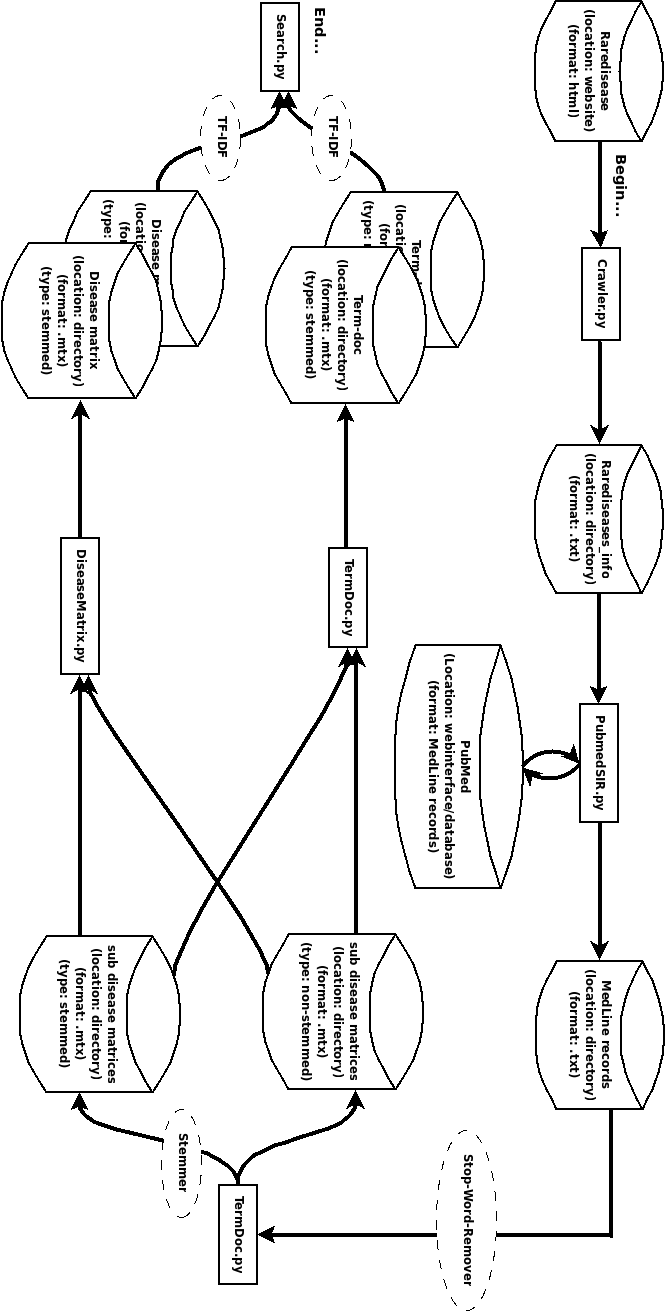
\includegraphics[width=1.0\textwidth]{diagrammer/system_overview_rotate.png}
        \end{center}
        \caption{Overview diagram of the system}
        \label{OverviewDiagram}
\end{figure}

\section{Modules}

In this section, we will go through the individual modules described
in section \ref{SystemOverviewAndDesign}. We will be giving an
overview of the module, its parts and the way that the data, in
between the modules, is structured. We will also be looking at the
filter modules, the auxiliary modules and the modules used for data
analysis.

\subsection{Crawler\label{Crawler}}

\subsubsection{Overview and Purpose}
The crawler is the first step in creating a database of MedLine
records, containing information about rare diseases, since its main
purpose is to gather information about what to search for in PubMed.

As described in \ref{Rarediseases_info}, Raredisease.info contains a
list of rare diseases and a varying degree of information on each
specific disease. We were referenced to the website by Henrik L.
J\o rgensen \cite{TheDude}. A Crawler to collect information from the
site, was the first module to be made. The crawler goes through every
disease from A to Z and 0-49 and saves the names of the diseases and
(if any exist) the synonyms, the specialized search string for PubMed
and a description of the disease. This information is then used by a
SIR-module which is described in the following section \ref{SIR}.

Our main module is named \textit{DiseaseCrawler}. It crawls the
Rarediseases.info webpage and gathers information as described
above. It is a rather large module since it has to take a series of
anomalies into account when crawling Rarediseases.info (like
dysfunctional subpages, strange characters and unexpected
white-spaces). It utilizes the auxiliary modules \textit{TextCleaner}
and \textit{IOmodule}, described in section \ref{AuxModules}.


\subsubsection{Methods and data description}
The crawler accepts a list of letter for which to gather information
from, e.g. ['A'] means gather all diseases beginning with A. It
utilizes the HTML parser library Beautifulsoup \cite{BS} to parse the
webpages, looking for disease names, synonyms, handcrafted searches
and uids. The crawled data is all stored in database of dictionaries
on the form:

\begin{center}
{\small
\{'terms': '', 'desc': '', 'db': u'omim', 'syn': [u'Pectus excavatum', u' macrocephaly and dysplastic nails', u'Familial short stature', u' developmental delay', u' pectus abnormalities', u' distinctive facies', u' and dysplastic nails'], 'uid': u'600399'\} 
}
\end{center}

The name of the file, that each of the datasets are stored in, is the
name of the disease. The above shows a example for the disease 'Zori
Stalker Williams syndrome'. The key 'terms' will contain the
handcrafted search string for PubMed if one is found while 'desc'
contains the description of the disease if one is available
(unfortunately on Rarediseases.info only 6.94\% contains one). 'db'
represents the choice of database to use and refers to either PubMed
or OMIM in our current cases. It is needed to know how to search for
the disease in Entrez, as described in the following section. 'syn' is
a list containing the various synonyms associated with the disease and
used for finding more relevant information about the disease. 'uid' is
a unique identifier found on all OMIM links and in some cases on
pre-calculated pubmed searches.

\subsection{SIR (Search and Information Retrieval)\label{SIR}}

\subsubsection{Overview and Purpose}
The \textit{PubmedSIR}-module reads in the information saved by the crawler (or any
other crawler). It uses Entrez for accessing, searching and retrieving
MedLine records from PubMed. The information contained within the
MedLine record represents our knowledge base about the diseases. The
\textit{PubmedSIR}-module is set to search in such a way that we hope to optimize
getting records that are actually relevant to the given disease. A
maximum of 500 Medline records are downloaded per disease using a two
phase search, all containing an abstract.

The main module is called \textit{PubmedSIR} and is used to search and
retrieve MedLine records from the PubMed database.

As mentioned above the searching is split into two phases where it
looks for at most 250 MedLine records in each phase. It first examines
whether there is a handcrafted search string to search for or whether
the disease has a PubMed or OMIM unique-id (uid). When searching for
the handcrafted search string, \textit{PubmedSIR} automatically adds the
additional search options ``AND hasabstract[text]'' to the string. This
makes sure that all the MedLine records, that are returned, contains
an abstract. This is unfortunately not possible when dealing with
PubMed/OMIM uids which means that we have to employ other means to
ensure that the returned MedLine records contains an abstract. This is
done by the method \texttt{getMedLineList} which takes a list of
PMIDs, downloads them from PubMed and runs through all the MedLine
records, selecting only those containing an abstract. Making a local
cleaning to ensure that the MedLine records contain abstracts also
means that we can not guarantee 500 MedLine abstracts for a disease
even thought they are available. This is a minor fault in our system
that should have been corrected if time allowed it but we have chosen
to continue with the information we have available. Alternatively
additional search options could be to also include constraints for
getting only abstracts in english, only records published after a
certain date etc. For options see the site PubMed help search
\cite{PubmedHelpSearch}

PubmedSIR relies primarily on the function
\textit{getArticleIDsFromMultipleSources} for searching across the two
major databases of Entrez - PubMed and OMIM. We have chosen not to
remove duplicate MedLine records between the first and second phase of
the search because it is our belief that if a record is present in
both searches, the terms is worth counting twice. The searches are
done as the described below.

First phase of the search:
\begin{itemize}

\item Search for term if it is present, OR

\item Search for pubmed/omim uid.

\item If we have obtained less than 250 MedLine records,
  
\begin{itemize}

  \item Search for the disease name on pubmed.

  \item Eliminate duplicates.

  \end{itemize}
\end{itemize}

Second phase of the search:
\begin{itemize}

\item Calculate all possible combinations of the synonyms.

\item Search for the combined synonym. If a combination returns 0
  results then eliminate all future searches that contains this
  combination since pubmed put in 'AND' between search terms ( meaning
  that future searches containing this combination will also return 0
  results).

\item Fill up until we get at most 500 MedLine records.

\end{itemize}

\subsubsection{Method and data description}
The primary function of the module is \texttt{gatherOfAllThings},
which reads in the information that were saved by the crawler. This
information is passed onto \texttt{getArticleIDs} that in turn calls
\texttt{getArticleIDsFromMultiSource} which searches the items
specified within the disease dictionary. \texttt{getArticleIDs} is also the
function that keeps track of the number of MedLine records that are
downloaded for each disease.

A typical dictionary read in from the crawler looks as follows:

\begin{center}
{\small
\{'disease x': \{'syn' : [xx, yy, zz], 'term' : string, 'uid' : string,
    'description' : string, 'db' : pubmed|omim\}, 'disease y': \{'syn' :
    [aa, bb], 'term' : string, 'uid' : string, 'description' : string,
    'db' : pubmed|omim\}, ...\}
}
\end{center}

\texttt{gatherOfAllThings} completes by performing a writeout of the MedLine
records to the disk in the following format:

\begin{center}
{\small
\{'disease a': [pmid1, pmid2, pmid3...], 'disease b' : [pmidx,
    pmidy,...], ...\}
}
\end{center}

The \textit{PubmedSIR} module uses the following auxillary modules (see
section\ref{AuxModules}):
\begin{itemize}
  \item \textit{SearchTermCombiner} which is a simple module that is used to
combine search terms in all of its possible unique combinations.
  \item \textit{IOmodule} handles Input/Output.
  \item \textit{TextCleaner} is used to sanitize the input strings.
\end{itemize}

For more information about the gathered dataset, see section \ref{Database}.

\subsection{TermDoc\label{TermDoc}}

\subsubsection{Overview and purpose}
The information gathered from the \textit{PubmedSIR}-module now needs to be
processed to allow queries to be made on it. An often used method in
Information Retrieval (IR) is the vector space model \ref{VectorSpace}
that represents the gathered information as document vectors (in a
term document matrix). The result is that queries to the system can be
made using a query vector, getting a similarity score/measure against
all documents contained within the model. In the following, we will go
through the creation of the sub term document matrices, the large term
document matrix and the compressed disease matrix.

We use a two-phase approach to construct the complete term document
matrix.

In the first phase, we make a sub term document matrix for each
disease containing the information from the MedLine records. We split
up the abstract, title and MeSH terms if present. Various filters can
be applied to the terms, e.g. stemming and stop word removal. We
choose to remove any kind of punctuation and the like because
otherwise the terms remain very noisy ("blood" and "blood." would be
two different terms). We keep single letters (except for 'a' which
counts as a stop word), because many diseases contains single letters
as identification of which type they are, e.g. 'Hemoglobin C
disease'. It is an fault in our system that we do not keep 'a', but it
was found to late.

The second phase simply goes through the sub term document matrices
and fill the term count values into complete term document matrix.

There are two main modules. The first, called \textit{TermDoc}, is
able to make sub term document matrices from a folder containing
MedLine records and to combine a folder containing sub term document
matrices into a complete term document matrix. The second one is
called \textit{DiseaseMatrix} and makes a matrix with disease vectors
instead of document vectors.

\subsubsection{Method and data describtion}
The main function for creating the sub term document matrices from a
folder containing MedLine records is
\texttt{medlineDir2MatrixDir}. This function requires a hash table
containing hashes for all the terms and pmids of the MedLine
record. The need for hash tables comes from the fact that the data
structures, we have chosen, does not support string entries. So hashes
can be made by the \texttt{createTermAndPmidHashes}. This function
goes through a folder containing MedLine records, while building a
term and pmid hash table. When \texttt{medlineDir2Matrix} has read in
the hash, it proceeds by calling \textit{gatherMatrixData} on each
file within the MedLine record folder. \texttt{gatherMatrixData}
extracts information from the file by the use of the auxillary module
\textit{RecordHandler} (see section \ref{AuxModules}). The information
can be specified by the user --- title, abstract and MeSH terms are
chosen by default, as these seem to give a good overall description of
a disease. This is also the place to perform stop word removal and
stemming. We have chosen to create both a stemmed and an unstemmed
matrix in order to test what performs best. \texttt{medlineDir2Matrix} then
calls \texttt{populateMatrix} with the data from
\texttt{gatherMatrixData}. This creates and returns a term document
matrix. Last it calls \textit{IOmodule} (see section \ref{AuxModules}) to write
the created term document matrix to the disk in Matrix Market format
(see section \ref{MatrixMarket}).

For creation of the large term document matrix, the function
\texttt{createTermDoc} is used. This goes through the folder containing
the sub term matrices and places the term count for each of the
MedLine records in the right place in the term document matrix. This
is basically done by looking up in the hash table for were to place
them. If the same MedLine record exists in two different diseases, the
term counts are summed. When done, it is written to the disk in Matrix
Market format.

The disease matrix is created by calling
\texttt{constructDiseaseMatrix} with a folder of sub term document
matrices as input. It then runs through every of the sub term document
matrices and calls \texttt{getColumnSum} for each of them. This sums
the sub-matrices to a single vector and returns one row for each of
the diseases which can be used to represent it. \texttt{getColumnSum}
has the option of making the average column sum instead of just
summing them. This option can be used to normalize the disease
vectors, should it be needed. The disease matrix is, like the term
document matrix, based on hash tables. These can be created by running
\texttt{createDiseaseHash} on a folder containing sub term document
matrices.

The \textit{TermDoc} module uses the following auxillary modules (see
section \ref{AuxModules}):

\begin{itemize}
  \item \textit{RecordHandler}, which is used for extraction with the
    records contained within the MedLine records, e.g. 'AB' for
    abstract etc.
  \item \textit{FilterInterface} used to get access to Porter stemmer and stop
word removal of string.
  \item \textit{IOmodule} and \textit{TextCleaner} as mentioned in the
    previous section.
\end{itemize}

\fxnote{evt lidt statestik}

\subsection{FilterInterface and heuristics}

\subsubsection{Overview and purpose}
When dealing with the amounts of information, in a system like this,
there is a need to make some modifications to the data. We choose to
sanitize the input information to our system by removal of
punctuations, commas, etc. and by making every term lowercase. This
helps reduce the number of different terms in the system. This has the
side-effect that it also removes punctuations within describtion of
e.g. chromosome errors. Taking an example, the string "1q42.4-qter
duplication" will be split into '1q42', '4', 'qter' 'duplication'. We
do, however, not consider this to be a problem since the query
recieves the same preprocessing as the term document matrix and it
should still be possible to retrieve the right
information\footnote{Using regular expression, it is possible to
  preserve the above string as: '1q42.4-qter', 'duplication' but we do
  not believe it important for the prototype}. The simple string
cleaning also allows the user to use other notations for the same
gene\footnote{'1q42.4-qter' and 1q42-4-qter amounts to the same}.

Another common technique in IR is to use stop word removal. This is
because words like 'this', 'the' and 'a' are very common and thereby
do not contain any information in the term-independent vector space
model. In some circumstances it is also normal to remove single letter
characters but as some diseases are characterized by having a special
type (as mentioned in \ref{TermDoc}), we choose not to remove single
letters. However, our stop word remover unfortunately does remove 'a'
due to its frequency in the English language. As mentioned earlier we
did not have time to correct this error.

\fxnote{evt lidt statestik}

\subsubsection{Some numbers about filtering}
Making a 'raw' term document matrix, without any filtering results in
1,945,966 terms. After sanitizing the information there are 465,220 terms 
and after stemming there is a further reduction to 390,766 terms.
There are a couple of modules involved with filtering. We have made a
\textit{FilterInterface} module to provide easy access to the different
filters.

\subsubsection{FilterInterface}
This is simply a gateway to various filters that are implemented in
separate modules. It is designed to return e.g. a stemmer or a stop
word remover that can be run on the abstracts before the term document
matrix is constructed. In the current prototype, it contains the
modules \textit{StopwordRemover}, \textit{Stemmer} and
\textit{TFIDFMatrix}.

\subsubsection{StopwordRemover}
The stop word remover allows for list of stop words to be supplied by
the user. By default it uses the nltk.corpus.stopwords of english stop
words which contains 127 stop words. There are other languages present
in the stop word corpus for a total of 2431 words, e.g. German,
Danish, Swedish, Norwegian and others. We do not know if any important
words are removed due in a multi language stop word removal. We assume
that most of our information is in English and have chosen only to
remove English stop words. It is possible to setup additional options
within the \textit{PubmedSIR} module (section \ref{SIR}) so that it will
only gather MedLine records containing abstracts in english but this
is preserved for a later version of the system.

\subsubsection{Stemmer}
To preserve flexibility our system allows another stemmer to be sent
to the function replacing the default stemmer. The default stemmer is
\textit{nltk.PorterStemmer().stem} that performs stemming on our
abstract, title and MeSH terms to ``smooth'' out the terms. It is only
advisable to run the stemmer after the stop word remover. This is
mainly because the stemmer changes some stop words so that they will
not be recognised by the stop word remover, e.g. performing stemming
on 'this' results in 'thi' which is not included in the default stop
word corpus.

\subsubsection{TFIDFMatrix}
The \textit{TFIDFMatrix} module is used to perform the TF-IDF
transformation of a term document matrix using the equation from
section \ref{TFIDF}. It performs the transformation by reading the
term frequency (tf) from an original matrix only containing term
counts and then by making a log-transformation of the tf. For finding
the inverse document frequency (IDF), we have made a precalculated
hash table containing the number of documents that the different terms
are present in such that $\mathit{idf} = \frac{D}{\sum_{d\prime =
    1}\delta_{d\prime w}}$. We then store the calculation of
$\mathit{tf} \cdot \mathit{idf}$ at the terms position within the term
document matrix. The transformed term document matrix is then saved to
the disk. The module then performs normalization of the document
vector to make sure that each document has the same influence on the
result of a query (and is used for the enhancing the speed of the
cosine similarity calculation described in section
\ref{VectorSimilarity}). The normalization is done as usual vector
normalization $\frac{\overrightarrow{a}}{||a||}$.

\subsection{Auxillary modules\label{AuxModules}}

Auxillary modules are used by the different modules to perform tasks
like input/output, stemming, stop word removing, cleaning text string
or combining synonyms into search queries.

\subsubsection{IOmodule}
Performs various I/O function. For instance when a module is writing
or reading objects like hash tables to/from the disk, it simply calls
the \texttt{pickleIn} or \texttt{pickleOut} function with a path. The
object is then written or read. It is also able to return a sorted
list of file references from a folder which is very useful when one
needs to keep track on how far the process has come. This module also
allows for term document matrices to be written or read from the disk
using the Matrix Market format (see section\ref{MatrixMarket}).

\subsubsection{TextCleaner}
This module performs string manipulation like removing tags from HTML
code, sanitizing strings for punctuation, commas and all other special
characters, decoding various HTML characters. Most of these task are
obtained by return a regular expression for the specific task.

\subsubsection{RecordHandler}
The \textit{RecordHandler} module is used to read information fields
from MedLine records which it returns as a dictionary containing the
requested fields.

\subsection{SearchInterface}
The search interface implements different approaches of measuring
similarity/distance between the query vector and document vector in
our term document matrix. Our two choices of measure in the vector
space model is the cosine similarity measure and a simple sum
measure. Instead of going through all the rows (documents) in our
matrix, we take the terms from the query vector and look up the only
the documents containing one or more of the queried terms. This limits
our search space and significantly enhances the time it takes to
process a query.

\subsubsection{SearchInterface}
This is the simple search interface that allows the different search
methods to be called, hence acting as a gateway like the
\textit{FilterInterface} described earlier.

\subsubsection{CosineMeasure}
This module is used to perform a search using the cosine measure for
distance calculations between the query vector and the rows of our
term document matrix. It uses \textit{SearchTermDoc} to get the row
indices of which rows the query terms are present in. It then sums up
the scores in accordance to the occurrence of the query term. This
should resemble usual cosine measuring between vector when performed
on a pre-normalized vector space (see section \ref{VectorSimilarity}).

\subsubsection{SumMeasure}
The \textit{SumMeasure} module is used to perform a different kind of
measure. It performs a summing of the entries in the in the document
vector according to the terms of the query vector. It basically acts
as the cosine measure but is used on a vector space that is not
normalized. Again note that the reason we can compare the two measures
is because of the simplifications made in \ref{VectorSimilarity}.

\subsubsection{SearchTermDoc}
This module is used as a support module for performing searches. Given
a search vector, it will return the row indices of the term document
vectors that contain any of the terms. It can extract the term columns
with the relevant documents indices and it can create the hashes
needed for normalization and for column element counts. It is also
performs reverse look up of pmids (documents) given a pmidhash value.

\subsection{Data analysis tools}

In order keep track of the amount of information that we have
collected, we have made a ``crude'' module for gathering information. It
can be used to get the total number of pmids including duplicates, the
number of MedLine records containing a title or the number of diseases
that contains a description. In addition to this, we made a module to
perform hierarchical clustering of the diseases of top 20 results
returned by our system.

The modules, that are part of the data analysis suite, is
\textit{Cluster} which performs the clustering,
\textit{DistanceMeasure} which implements different
distance/similarity measures to be used within \textit{Cluster} and
\textit{Stat} which is able to count various information fields
contained within the MedLine records.

\subsubsection{Cluster}
The \textit{Cluster} module contains various functions in relation to
hierarchical clustering and drawing of dendrograms of the returned
clusters. The hierarchical clusterings has unfortunately not been made
as generic as it could be. For now, slight modifications are required
between running either on a disease matrix / term document matrix or a
sub term document matrix. We have no intentions of performing a full
clustering on a term document matrix, as it simply contains too many
entries to consider clustering - at least with the resources available
currently. The hierarchical clustering and dendrogram functionalities
are based on Collective Intelligence \cite{CollectiveIntelligence}
with slight modification to adopt it for our data.

\subsubsection{DistanceMeasure}
This module simply implements its own cosine measure functions for
sparse and dense matrices.

\subsubsection{Stat}
This module is able to count the various different fields within the
MedLine records, e.g. how many a title, a MeSH, etc. It is also
able to count how many duplicate pmids there is.

\section{The database\label{Database}}

Our raw dataset consists mainly of two parts that are gathered
independently. The first part is the information gathered from
Rarediseases.info. The files reside in a subfolder called
\textit{rarediseases\_info} containing 6881 text files. Looking into
one of these files it is possible to see exactly what information have
been used to retrieve the medline records for a specific disease. The
second part of our raw dataset is the information gathered from PubMed
by the \textit{PubmedSIR} module. This information can be find in the subfolder
\textit{medline\_records}. Again we have chosen to store it as plain
text files which enable the use of GNU unix/linux command line tools
for quick looks inside or using grep to look for specific words inside
a disease file.

Due to the limit on 500 abstracts per disease and with a total of
6,881 different rare diseases from Raredisease.info, the theoretical
upper limit on the number of abstract is 3,440,500. But since the
diseases are rare and the crawled information from Rarediseases.info
faulty at times, in reality the number of returned MedLine records is
much smaller. In fact, we only have 602,466 unique MedLine records
(about 2.8 million from the theoretical limit) and approximately
1,036,432 when counting duplicates. One of the MedLine records is even
shared among 240 diseases which indicates that it is an overview over
many diseases. There are also 505 diseases that do not return any
information at all. This means the remaining 6,376 diseases, on
average, have 94.49 MedLine records each. When searching PubMed, we
need to impose the 500-limit on the number of abstracts because (even
though the diseases are rare) some of them will return a lot of
information. Kidney cancer, though on the list of rare diseases, will
return 51,393 hits (\date{January 3, 2010}) with a search on PubMed
(only those with an abstract) and this is without considering any
synonyms or possibly handcrafted search terms.

We have choosen to remove the 505 empty disease entries from our
dataset because, without any information about these diseases, our
system will be unable to find/diagnose them.

\subsubsection{More statistics on the data}
Out of the 1,036,432 MedLine records, 1,036,417 has title. This is
nearly 100\% (99.99\%). Not all of the MedLine records have MeSH terms
although 924,026 has. This is 89.15\% of all the entries. \fxnote{This might
be a bit misleading as it count the duplicate ones too, try to get
count without duplicates.}

\section{Techincal conclusions}

When performing text mining, a robust is needed to be able to handle
various situations. This became apparent to us after having written
the first version of it. Due to the inconsistency of
Rarediseases.info, it crashed every time that it ran into a new
special case on Rarediseases.info. Therefore, when crawling website
based on incomplete topics like rare diseases, its important to make
proper error handling and logging which diseases were missed in the
first run since errors are near certainty. As a sidenote on this, the
BeautifulSoup module is a really useful tool when crawling HTML since
it is able to correct and prettify many common website errors.

Gathering data from PubMed was performed by the Entrez module which on
several occasions crashed. This gave birth to the need to gather the
MedLine records in chunks to be able to resume them at any point. When
collecting data from OMIM- or PubMed-uid links, there is no way to
ensure that the returned MedLine records contains abstract and this
needs to be dealt with locally (as mentioned in \ref{SIR}). Before
performing text or data mining, ALWAYS seek the permission of those
running the site or sites. During this project, we got banned from
Rarediseases.info once and from Orpha.net twice. This was not because
we broke any laws or rules but because most websites today protects
themselves from harmful bots, replay attacks and other risks to the
website. If you do not have permission to find information on the
website, at least make sure you give your credentials, browser type,
etc. with the crawler.

Constructing a term document matrix requires a sparse data structure
for being stored on disk and in memory but when working with document
vectors, making them dense can mean a huge speed up on arithmetic
operations. Choosing to rewrite some of the more computational parts
to a low level language like C would also increase performance. Saving
intermediate steps along the way while making term document matrices
also allows other preprocessing steps to be performed, if needed later
in the project and is recommendable for large projects.

When querying the matrices, it is important to try several different
methods since the most well known or obvious one, might not be the
best choice (as we shall see in the following chapter).


\chapter{Experiments and Results\label{ExperimentsResults}}

In this section, we introduce the test cases we intend to use. We go
through the details of our cosine and sum measure scoring schemes that
we will be using to test our systems ability to rank a correct disease
given a list of symptoms. This is followed by various test results
using different similarity measures and different matrix models. By
comparing the individual top scores of each measure on a given matrix,
stemmed or non-stemmed, we find the most efficient measure to score
data on our system. It should here be noted that each time we score a
given disease, we do it by taking the top 3000\footnote{A number
  chosen at random in between our total number of different diseases}
of the documents returned by the similarity measure and the Search
module. \\

We then look at ... Note: cluster and semantic section are still to
written. \\

Finally, we take discuss the potential noise of overview
articles\footnote{Articles found in / refering to many different
  diseases} and test the potential of concensus normalization.

\section{Test cases}

\textbf{BMJ} \\
In order to test our system we need to find some suitable test
cases that are not biased towards our own system. We have chosen to
first of all test our system against a subset of the disease cases in
\cite{HangwiTang11102006}, i.e. disease cases which can be found in
our system\footnote{As mentioned earlier in \ref{Database} our system
  can only help diagnose the diseases contained in the
  system}. However, there is one major difference between the tests
conducted by the people behind \cite{HangwiTang11102006} - they have a
medical background (a respiratory and sleep physician and a
rheumatologists) contrary to our computer science background. This
means that we have no bias or knowledge about selecting symptoms and,
as they explain, given some of the symptoms the correct diagnosis were
evident to them \cite{HangwiTang11102006}. Note that we will, in the
following sections, be reffering to the subset of the test cases in
\cite{HangwiTang11102006} as BMJ since this is were it was found. \\

The subset of the \cite{HangwiTang11102006} test cases include the
following 13 diseases:

\begin{table}[!h]
\caption{Disease / Symptoms list}
\begin{tabular}{|l|p{7cm}|}
\hline
Disease & Symptoms \\
\hline
Infective endocarditis & Acute, aortic,  regurgitation, depression,  abscess " \\
\hline
Cushing's syndrome & hypertension, adrenal, mass \\
\hline
Eosinophilic granuloma & Hip, lesion, older, child \\
\hline
Ehrlichiosis & fever, bilateral, thigh, pain, weakness \\
\hline
Neurofibromatosis type 1 & multiple, spinal, tumours, skin, tumours \\
\hline
Pheochromocytoma & hypertension, papilledema, headache, renal, mass, cafe, au, lait \\
\hline
Creutzfeldt-Jakob disease & ataxia, confusion, insomnia, death \\
\hline
Churg-Strauss syndrome & Wheeze, weight, loss, ANCA, haemoptysis, haematuria \\
\hline
Dermatomyositis & myopathy, neoplasia, dysphagia, rash, periorbital, swelling \\
\hline
Cat Scratch Disease & renal, transplant, fever, cat, lymphadenopathy \\
\hline
TEN & bullous, skin, conditions, respiratory, failure, carbamazepine \\
\hline
MELAS & seizure, confusion, dysphasia, T2, lesions \\
\hline
Brugada syndrome & cardiac arrest sleep \\
\hline
\end{tabular}
\end{table}

Orphanet
To examine significance of the test result, we have additionally selected some diseases at 'random' from Orpha.net. We require that the disease has a description on Orpha.net containing a sentence with 'characterized by'. Occationally we have meant that the 'characterized by' contained too many specific symptoms (e.g. derivatives of the name of the disease or a several sentences long list of symptoms) and have removed certain symptoms from the list. Examples of reductions would be\footnote{Note that this is based solely on our own judgement as non-physicians.} \\

congenital anomalies (microcephaly, specific facial characteristics, broad thumbs and halluces and postnatal growth retardation), intellectual deficit and behavioural characteristics

reduced to

congenital anomalies, intellectual deficit, behavioural

and 

congenital malformations: hydrocephalus (due to Dandy-Walker anomaly), cleft palate, and severe joint contractures

reduced to

congenital malformations: hydrocephalus, cleft palate, severe joint contractures

The test cases fetched from Orpha.net include the following 30 different diseases: \\

\begin{table}[h]
\caption{Disease / symptom list 2}
\begin{tabular}{| p{5.5cm} | p{5.5cm} |}
\hline
Disease name & Symptom list \\
\hline
Apparent mineralocorticoid excess & early-onset, severe hypertension, associated, low renin levels, hypoaldosteronism \\
\hline
Rubinstein-Taybi syndrome & congenital anomalies, intellectual deficit, behavioural characteristics \\
\hline
Aagenaes syndrome & chronic severe lymphoedema, severe neonatal cholestasis, lessens during early childhood and becomes episodic \\
\hline
Aase Smith syndrome & congenital malformations: hydrocephalus, cleft palate, severe joint contractures \\
\hline
Achondroplasia & short limbs, hyperlordosis, short hands, macrocephaly, high forehead and saddle nose \\
\hline
Acalvaria & missing scalp and flat bones over an area of the cranial vault \\
\hline
Acrodysostosis & abnormally short and malformed bones of the hands and feet (peripheral dysostosis), nasal hypoplasia and mental retardation \\
\hline
Acromegaly & progressive somatic disfigurement (face and extremities) and systemic manifestations \\
\hline
Biliary atresia & biliary obstruction of unknown origin, neonatal period \\
\hline
Bronchiolitis obliterans with obstructive pulmonary disease & inflammatory and fibrosing thickening of bronchiolar walls, airflow obstruction \\
\hline
Cholera & severe diarrhea and vomiting \\
\hline
Choroideremia & progressive degeneration of the choroid, retinal pigment epithelium (RPE), and neural retina \\
\hline
Coats disease & abnormal development of retinal vessels (telangiectasia) with a progressive deposition of intraretinal or subretinal exudates \\
\hline
Omphalocele cleft palate syndrome lethal & omphalocele and cleft palate \\
\hline
Darier disease & keratotic papules in seborrheic areas and specific nail anomalies \\
\hline
Ichthyosis hepatosplenomegaly cerebellar degeneration & ichthyosis, hepatosplenomegaly and late-onset cerebellar ataxia \\
\hline
Emery-Dreifuss muscular dystrophy & muscular weakness and atrophy, with early contractures of the tendons and cardiomyopathy \\
\hline
\end{tabular}
\end{table}

\begin{table}[h]
\caption{Disease / symptom list 2, continuet}
\begin{tabular}{| p{5.5cm} | p{5.5cm}|}
\hline
Costello syndrome & postnatal growth retardation, coarse facies, intellectual deficit, skin anomalies and cardiac abnormalities \\
\hline
Fibrodysplasia ossificans progressiva & congenital malformation of great toes, progressive, disabling heterotopic osteogenesis in predictable anatomical patterns \\
\hline
Acropectorovertebral dysplasia & fusion of the carpal and tarsal bones, with complex anomalies of the fingers and toes \\
\hline
Osteogenesis imperfecta & increased bone fragility and low bone mass \\
\hline
Primary biliary cirrhosis & injury of the intrahepatic bile ducts \\
\hline
Hennekam syndrome & lymphoedema, intestinal lymphangiectasia, intellectual deficit and facial dysmorphism \\
\hline
Hyperlysinemia & elevated levels of lysine in the cerebrospinal fluid and blood \\
\hline
Jackson-Weiss syndrome & tarsal and/or metatarsal coalitions and variable craniosynostosis, accompanied by facial anomalies, broad halluces and normal hands \\
\hline
Jalili syndrome & amelogenesis imperfecta and cone-rod retinal dystrophy \\
\hline
Jeune syndrome & narrow thorax and short limbs \\
\hline
Multiple myeloma & overproduction of abnormal plasma cells in the bone marrow and manifested by skeletal destruction, bone pain, and presence of abnormous immunoglobulins \\
\hline
Trichodental syndrome & fine, dry and short hair with dental anomalies \\
\hline
\end{tabular}
\end{table}

\textbf{Blind tests}
In addition to the BMJ and Oprhanet test cases, we have performed a blind test on disease cases given by physician \cite{TheDude}.
>>Finish this section when ordentlig-syg results arrive!<<

\subsection{4.2 Scoring schemes}

As mentioned in the previous chapters, we will employ two different kinds of scoring measures - the cosine and sum measure. The original idea, behind using a sum measure, was to test how much the cosine measure would outperform this simpler measure but as we shall see in \ref{TestingCosineSimilarity} and \ref{TestingSumSimilarity}, the cosine measure is actually outperformed itself by the sum measure. We will try to explain this 'oddity' in the given section and for now focus the way we use the two different kinds of measure. The following cosine and sum score measures are described in accordance to how they function on the term document matrix. The exception of the disease matrix is described at the end of this section.\\

\subsubsection{4.2.1 The cosine score\label{CosineScore}}

We will be testing the following three different approaches to using
the cosine similarity measure: cosine mean, cosine median and cosine
max.\\

\textbf{Cosine mean}  \\
Every disease has one or more documents attached to it (as
described in \ref{Database}). This means that the same disease might
be returned many times when looking at a top score of document
similarity measures produced by e.g. the cosine score. Therefore, to
give each disease a score, we use a form of concensus method where we
sum the scores of each document belonging to that disease. This
produces a mean score of each disease. \\

When the system (or more specifically the Search module) receives a
query, it ranks the query vector of terms against all document vectors
in which one or more of the terms has appeared. This results in a list
of scores $\mathbb{x} = \left\{x_1, x_2, \dots, x_n \right\}$. It then
runs through every scored document and adds the score to the disease
from which the document came (in accordance to the concensus method
just described). Since some documents appear in more than one disease
(\ref{Database}), several diseases might have the sum of a single
document added to its score $\mathbb{x}_{\textrm{disease}_{1}} =
\left\{x_{\textrm{sum for} x_2, x_7, x_i, \dots, x_j}\right\}$,
$\mathbb{x}_{\textrm{disease}_{2}} = \left\{x_{\textrm{sum for} x_1,
  x_2, x_9, \dots, x_47, x_n}\right\}$.  Lastly, we evaluate the total
ranking of each disease. We combine each $x_{\textrm{disease}_1}$,
$x_{\textrm{disease}_2}$ into a list of all the returned disease
$\mathbb{SL} = \left\{x_{\textrm{disease}_1},x_{\textrm{disease}_2},
\dots, x_{\textrm{disease}_n}\right\}$. These are then sorted and the
highest scoring is deemed the most likely to be the correct disease
given the query vector. \\

\textbf{Cosine median}
The median is calculated much like the mean, except for selecting the median of $\mathbb{x}_{\textrm{disease}_{1}} = \left\{x_2,x_7, x_i, \dots, x_j\right\}, \mathbb{x}_{\textrm{disease}_{2}} = \dots, \mathbb{x}_{\textrm{disease}_{n}}$, instead of summing the scores as we did above. \\

\textbf{Cosine max} \\
Does the same as above, just selects the maximum scoring in each disease lists and sort the resulting list and select the highest scoring as the most probable. \\

\subsubsection{4.2.2 The sum score}

The sum measure works exactly like the cosine mean measure, except for running on non-normalized vectors. See \ref{VectorSimilarity} and \ref{SimpleSum} for further reasoning. \\

\subsubsection{4.2.3 The disease matrix exception}

This is simply a short note on how we use the cosine and sum measures on the disease matrix. The disease matrix has no document vectors and is solely made up of summed disease vectors. This means that there is no point in using cosine mean, median or max, as there is no multiple label occurences to run a concensus method over. Here the score is simply the cosine or sum measure calculated for each of the diseases that contain the queried term(s). \\

\subsection{4.3 Testing the cosine similarity measure\label{TestingCosineSimilarity}}

The first test we run is on for the three different cosine scoring measures - mean, median and max. On the two barcharts below \ref{termDoc_bmj_hist_3000_ns_mea_med_max_nc} and \ref{termDoc_orphan_hist_3000_ns_mea_med_max_nc} are shown the query scores of the BMJ and the Orhpa.net test cases. These are run on the non-stemmed term document matrix. The scores a drawn on a logarithmic scale while the 'real' scores a shown below each chart. Note that the values are 0-indexed(!) and all tests are performed on TF-IDF preprocessed matrices. \\


\begin{figure}[h!]
        \begin{center}
          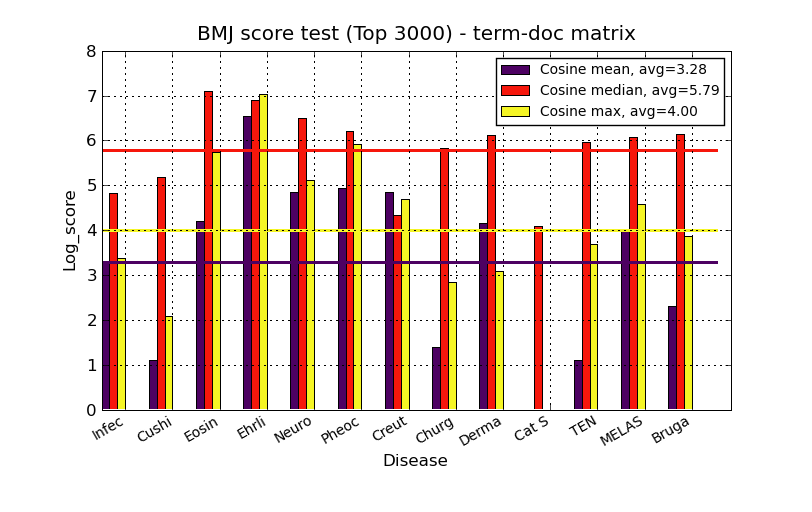
\includegraphics[width=0.9\textwidth]{termDoc_bmj_hist_3000_ns_mea_med_max_nc.png}
        \end{center}
        \caption{Test of non-stemmed mean, median and max using normalization and cosine}
        \label{termDoc_bmj_hist_3000_ns_mea_med_max_nc}
\end{figure}

 
Cosine: mean - Scores: [25, 2, 66, 692, 128, 139, 128, 3, 63, 0, 2, 52, 9] - In top 20: 5 \\
Cosine: median - Scores: [123, 179, 1210, 1004, 665, 502, 76, 343, 455, 59, 392, 430, 464] - In top 20: 0 \\
Cosine: max - Scores: [28, 7, 311, 1123, 166, 375, 109, 16, 21, 0, 39, 96, 47] - In top 20: 3 \\


\begin{figure}[h!]
        \begin{center}
          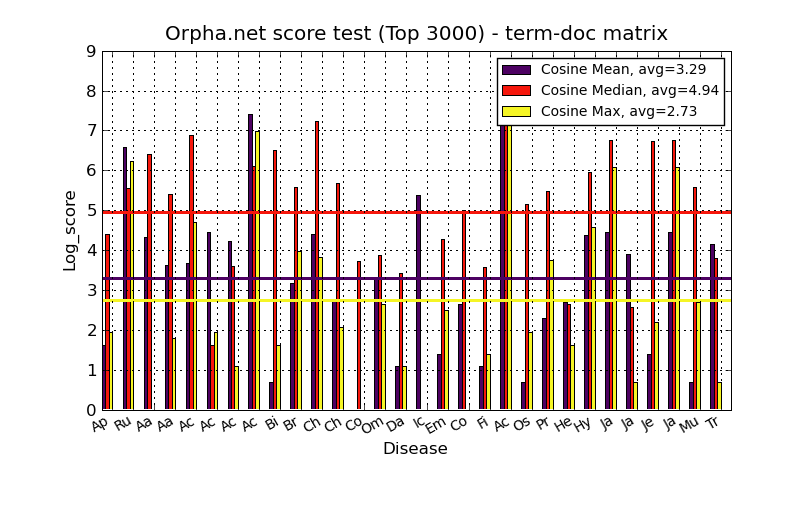
\includegraphics[width=0.9\textwidth]{barcharts/termDoc_orphan_hist_3000_ns_mea_med_max_nc.png}
        \end{center}
        \caption{Test of non-stemmed mean, median and max using normalization and cosine}
        \label{termDoc_orphan_hist_3000_ns_mea_med_max_nc}
\end{figure}
 
Cosine: mean - Scores: [4, 664, 30, 47, 38, 85, 62, 1371, 1, 32, 83, 15, 0, 26, 2, 81, 3, 16, 2, 3000, 4, 10, 13, 24, 66, 35, 3, 66, 4, 34] - In top 20: 13 \\
Cosine: median - Scores: [163, 357, 76, 240, 948, 4, 76, 141, 384, 314, 505, 211, 44, 181, 42, 773, 87, 169, 189, 3000, 179, 265, 21, 491, 692, 37, 435, 692, 358, 233] - In top 20: 1 \\
Cosine: max - Scores: [4, 858, 0, 10, 44, 15, 2, 541, 4, 116, 99, 18, 0, 6, 2, 0, 22, 0, 3, 3000, 9, 67, 5, 63, 201, 1, 8, 201, 9, 0] - In top 20: 19 \\

As we see here, the mean cosine measure performs best in the BMJ test set while the max cosine measure scores best in the Orpha.net test set. The median measure has an overall low score and running some quick tests on the different matrices, quickly reveals that median is not well suited as a measure to take into consideration. Therefore we will not be testing further on the cosine median score and continues with the two remaining scores from here on. Note that the AC score that has the worst performance in the Orpha.net test. It can and will happen that diseases are not found within the top 3000 documents that is returned. When this is the case, to avoid confusion in the bar charts and statistics, we simply set the score of any disease not found to a the high value of 3000, representing a bad performance. Note also that a missing bar, represents the top score 0. \\

We now continue testing the scoring measures, this time comparing the non-stemmed and stemmed term document matrices. The results are shown in the figures \ref{termDoc_bmj_hist_3000_ns_mea_s_mea_ns_max_s_max} and \ref{termDoc_orphan_hist_3000_ns_mea_s_mea_ns_max_s_max} below.

\begin{figure}[h!]
        \begin{center}
          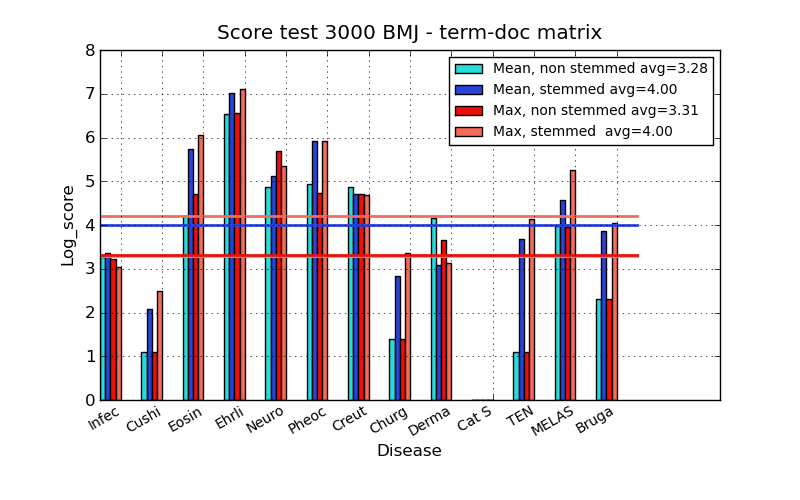
\includegraphics[width=0.9\textwidth]{barcharts/termDoc_bmj_hist_3000_ns_mea_s_mea_ns_max_s_max.png}
        \end{center}
        \caption{Test of non-stemmed mean, median and max using normalization and cosine}
        \label{termDoc_bmj_hist_3000_ns_mea_s_mea_ns_max_s_max}
\end{figure}

Cosine: mean non-stemmed - Scores: [25, 2, 66, 692, 128, 139, 128, 3, 63, 0, 2, 52, 9] - In top 20: 5 \\
Cosine: mean stemmed - Scores: [24, 2, 110, 710, 292, 113, 110, 3, 38, 0, 2, 51, 9] - In top 20: 5 \\
Cosine: max non-stemmed - Scores: [28, 7, 311, 1123, 166, 375, 109, 16, 21, 0, 39, 96, 47] - In top 20: 3 \\
Cosine: max stemmed - Scores [20, 11, 427, 1232, 210, 370, 108, 28, 22, 0, 62, 192, 56] - In top 20: 2 \\

\begin{figure}[h!]
        \begin{center}
          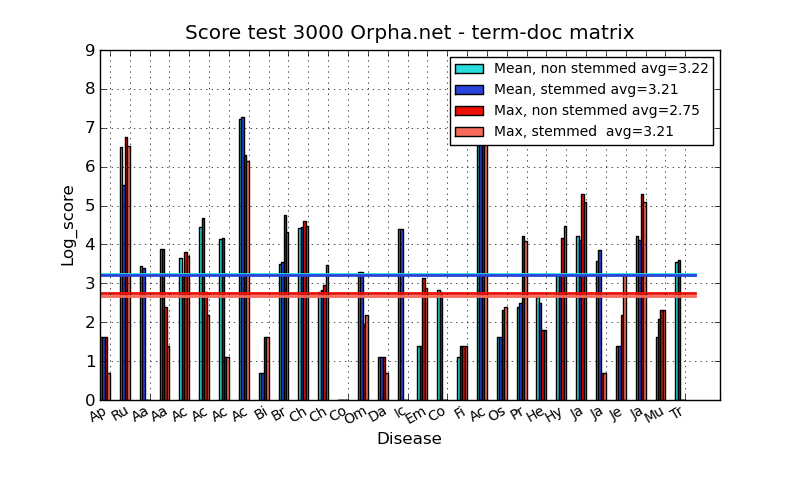
\includegraphics[width=0.9\textwidth]{barcharts/termDoc_orphan_hist_3000_ns_mea_s_mea_ns_max_s_max.png}
        \end{center}
        \caption{Test of non-stemmed mean, median and max using normalization and cosine}
        \label{termDoc_orphan_hist_3000_ns_mea_s_mea_ns_max_s_max}
\end{figure}
 
Cosine: mean non-stemmed - Scores: [4, 664, 30, 47, 38, 85, 62, 1371, 1, 32, 83, 15, 0, 26, 2, 81, 3, 16, 2, 3000, 4, 10, 13, 24, 66, 35, 3, 66, 4, 34] - In top 20: 13 \\
Cosine: mean stemmed - Scores: [4, 248, 29, 48, 23, 106, 64, 1436, 1, 34, 85, 16, 0, 26, 2, 81, 3, 15, 3, 3000, 4, 11, 11, 24, 60, 46, 3, 60, 7, 36] - In top 20: 13 \\
Cosine: max non-stemmed - Scores: [4, 858, 0, 10, 44, 15, 2, 541, 4, 116, 99, 18, 0, 6, 2, 0, 22, 0, 3, 3000, 9, 67, 5, 63, 201, 1, 8, 201, 9, 0] - In top 20: 19 \\
Cosine: max stemmed - Scores: [1, 677, 0, 3, 40, 8, 2, 462, 4, 75, 87, 31, 0, 8, 1, 0, 17, 0, 3, 3000, 10, 58, 5, 86, 162, 1, 24, 162, 9, 0] - In top 20: 18 \\

The two score tests just performed now presents us with a dilemma. In the BMJ test set the 'mean stemmed' and 'non-stemmed' scores performs best while in the Orpha.net test set, it is just the opposite. We have chosen to cope with this by taking out the top score measure for each of the test sets - 'mean non-stemmed' from BMJ and 'max stemmed' from the Orpha.net. \\

The next step is to analyse our data a bit by performing a square root transformation \ref{SquareRoot} of the TF-IDF preprocessed data above. Note that it is required that all values transformed are between 0 and 1, which in our case is secured by the fact that the matrices, we use for the cosine measure, are normalized. The reason for the square root analysis is that it allows us to see whether the data has been correctly weighted. The square root transformation raises small values by a greater degree than it does large values. This means that if our scores improve, the information containing terms in the term document matrix have not been given high enough values by the applied heuristics. \\

The tests are shown in the figures below, where we compare the best measures from above with their square root transformation.

\begin{figure}[h!]
        \begin{center}
          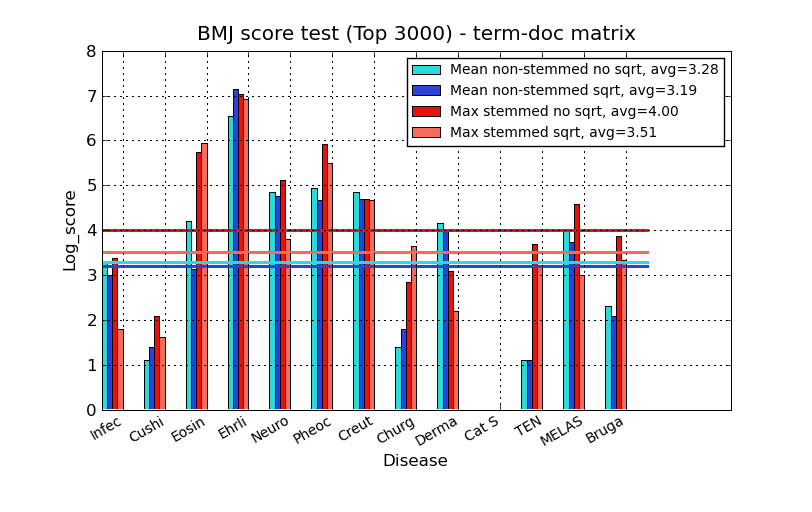
\includegraphics[width=0.9\textwidth]{barcharts/termDoc_bmj_hist_3000_ns_mea_ns_mea_sqr_s_max_s_max_sqr.png}
        \end{center}
        \caption{Test of non-stemmed mean, median and max using normalization and cosine}
        \label{termDoc_bmj_hist_3000_ns_mea_ns_mea_sqr_s_max_s_max_sqr}
\end{figure}

 
Cosine: mean non-stemmed - Scores: [25, 2, 66, 692, 128, 139, 128, 3, 63, 0, 2, 52, 9] - In top 20: 5 \\
Cosine: mean stemmed sqrt - Scores: [19,3,22,1268,115,105,108,5,54,0,2,41,7] - In top 20: 6 \\
Cosine: max non-stemmed - Scores: [20, 11, 427, 1232, 210, 370, 108, 28, 22, 0, 62, 192, 56] - In top 20: 2 \\
Cosine: max stemmed - Scores: [2, 10, 136, 1123, 68, 249, 130, 44, 8, 0, 47, 65, 25] - in top 20: 4 \\

\begin{figure}[h!]
        \begin{center}
          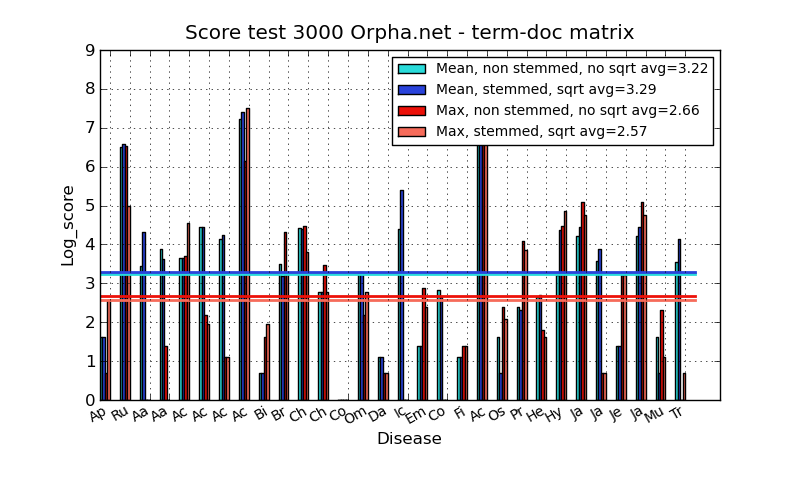
\includegraphics[width=0.9\textwidth]{barcharts/termDoc_orphan_hist_3000_ns_mea_ns_mea_sqr_s_max_s_max_sqr.png}
        \end{center}
        \caption{Test of non-stemmed mean, median and max using normalization and cosine}
        \label{termDoc_orphan_hist_3000_ns_mea_ns_mea_sqr_s_max_s_max_sqr}
\end{figure}

 
Cosine: mean non-stemmed - Scores: [4, 664, 30, 47, 38, 85, 62, 1371, 1, 32, 83, 15, 0, 26, 2, 81, 3, 16, 2, 3000, 4, 10, 13, 24, 66, 35, 3, 66, 4, 34] - In top 20: 13 \\
Cosine: mean stemmed sqrt - Scores: [4, 725, 75, 37, 38, 85, 68, 1651, 1, 23, 80, 15, 0, 26, 2, 218, 3, 13, 2, 3000, 1, 9, 14, 78, 84, 48, 3, 84, 1, 62] - In top 20: 13 \\
Cosine: max non-stemmed - Scores: [1, 677, 0, 3, 40, 8, 2, 462, 4, 75, 87, 31, 0, 8, 1, 0, 17, 0, 3, 3000, 10, 58, 5, 86, 162, 1, 24, 162, 9, 0] - In top 20: 18 \\
Cosine: max stemmed sqrt - Scores: [12, 145, 0, 0, 93, 6, 2, 1842, 6, 25, 44, 15, 0, 15, 1, 0, 10, 0, 3, 3000, 7, 46, 4, 128, 115, 1, 24, 115, 2, 1] - In top 20: 19 \\

These tests reveal some interesting results. Looking at the BMJ test set we see an overall improvement in the performance of the square root transformed measures. In Orpha.net test set there is an improvement in 'max stemmed' measure while a slight worsening of the 'mean non-stemmed' measure. However, there is no change in the number of top 20 results and the other measures shows a more significant improvement that the worsening of the last mentioned measure. Based on these results, we will not deny that the data in the TF-IDF matrices are not as optimized as could have been expected. But we can not say if these anomalies stem from the data or the calculations themselves. For now, we choose to view the square root transformation as a general improvement. \\

In section \ref{DiseaseMatrix}, we will be using the best measure of the cosine scoring tests executed above - the 'mean stemmed sqrt' and the 'max stemmed sqrt' cosine similarity measures. \\

\subsection{4.4 Testing the sum similarity measure\label{TestingSumSimilarity}}

In this section, we the same tests as described in the previous section, except for the square root transformation which makes no sense since we will be running on unnormalized data. Or in other word on values above and below 1 \ref{SquareRoot}. The first test is run for the mean, median and max sum measures on a TF-IDF non-normalized term document matrix. The results are shown on the figures \ref{termDoc_bmj_hist_3000_sum_mea_med_max} below. 

\begin{figure}[h!]
        \begin{center}
          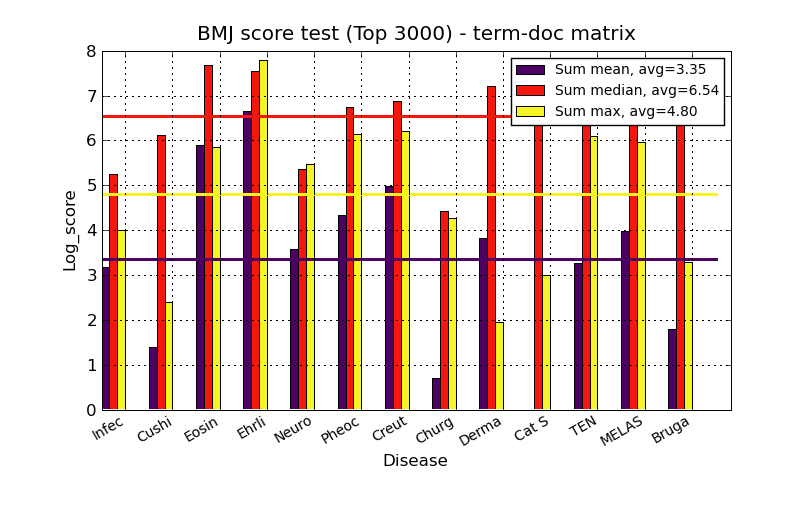
\includegraphics[width=0.9\textwidth]{barcharts/termDoc_bmj_hist_3000_sum_mea_med_max.png}
        \end{center}
        \caption{Test of non-stemmed mean, median and max using normalization and cosine}
        \label{termDoc_bmj_hist_3000_sum_mea_med_max}
\end{figure}

Sum: mean - Scores: [23, 3, 362, 772, 35, 76, 144, 1, 45, 0, 25, 53, 5] - In top 20: 4 \\
Sum: median - Scores: [188, 459, 2150, 1878, 213, 852, 974, 83, 1353, 670, 2193, 689, 1210] - In top 20: 0 \\
Sum: max - Scores: [54, 10, 344, 2401, 235, 469, 495, 70, 6, 19, 441, 391, 26] - In top 20: 3

\begin{figure}[h!]
        \begin{center}
          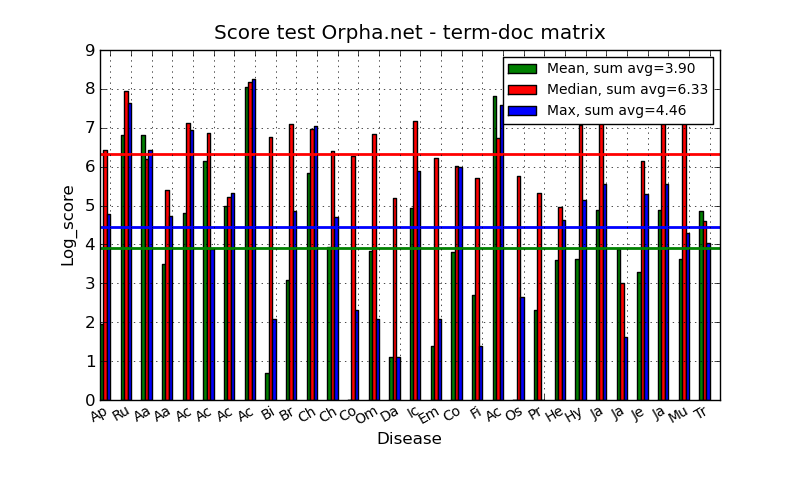
\includegraphics[width=0.9\textwidth]{barcharts/termDoc_orphan_hist_3000_ns_mea_med_max_sum.png}
        \end{center}
        \caption{Test of non-stemmed mean, median and max using normalization and cosine}
        \label{termDoc_orphan_hist_3000_ns_mea_med_max_sum}
\end{figure}
 
Sum: mean - Scores: [6, 910, 917, 32, 122, 460, 145, 3119, 1, 21, 342, 50, 0, 45, 2, 137, 3, 44, 14, 2458, 0, 9, 36, 37, 132, 47, 26, 132, 37, 127] - In top 20: 8 \\
Sum: median - Scores: [626, 2814, 495, 219, 1232, 963, 182, 3590, 872, 1207, 1056, 595, 526, 940, 179, 1292, 503, 408, 304, 845, 320, 204, 143, 1165, 1763, 19, 467, 1763, 1532, 100] - In top 20: 1 \\
Sum: max - Scores: [119, 2081, 611, 113, 1031, 48, 203, 3833, 7, 127, 1139, 109, 9, 7, 2, 357, 7, 401, 3, 1957, 13, 0, 102, 169, 260, 4, 198, 260, 72, 55] - In top 20: 9 \\

Like in the previous section, we again see the poor results given by the median measure and discards this for further testing. In the next test we compare the mean and sum measure in the stemmed and non-stemmed matrices. The tests are shown on the figures \ref{termDoc_bmj_hist_3000_ns_s_mea_max_sum} and \ref{termDoc_orphan_hist_3000_ns_s_mea_max_sum}.

\begin{figure}[h!]
        \begin{center}
          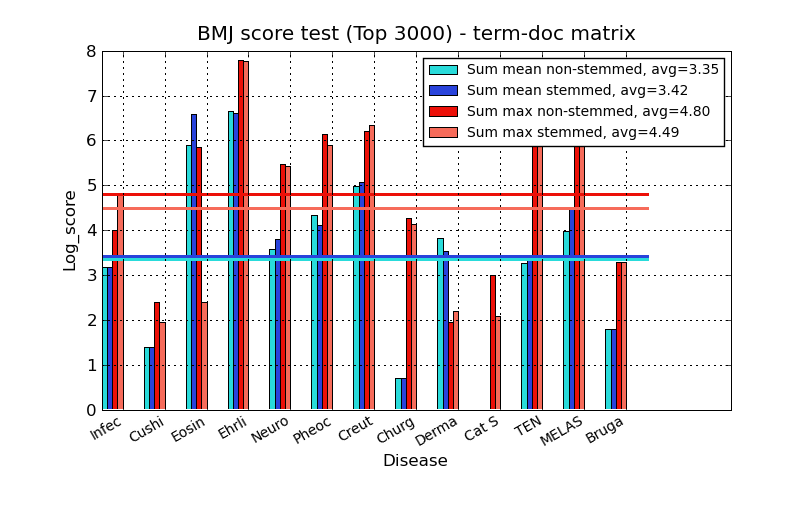
\includegraphics[width=0.9\textwidth]{barcharts/termDoc_bmj_hist_3000_ns_s_mea_max_sum.png}
        \end{center}
        \caption{Test of non-stemmed mean, median and max using normalization and cosine}
        \label{termDoc_bmj_hist_3000_ns_s_mea_max_sum}
\end{figure} 

Sum: mean non-stemmed - Scores: [23, 3, 362, 772, 35, 76, 144, 1, 45, 0, 25, 53, 5] - In top 20: 4 \\
Sum: mean stemmed - Scores: [23, 3, 720, 746, 44, 60, 158, 1, 33, 0, 27, 88, 5] - In top 20: 4 \\
Sum: max non-stemmed - Scores: [54, 10, 344, 2401, 235, 469, 495, 70, 6, 19, 441, 391, 26] - In top 20: 3 \\
Sum: max stemmed - Scores: [120, 6, 10, 2374, 228, 360, 566, 62, 8, 7, 394, 496, 26] - In top 20: 4

\begin{figure}[h!]
        \begin{center}
          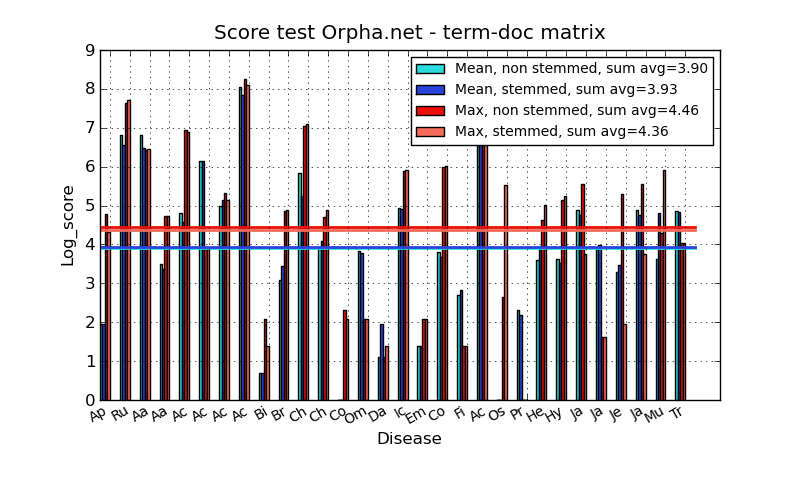
\includegraphics[width=0.9\textwidth]{barcharts/termDoc_orphan_hist_3000_ns_s_mea_max_sum.png}
        \end{center}
        \caption{Test of non-stemmed mean, median and max using normalization and cosine}
        \label{termDoc_orphan_hist_3000_ns_s_mea_max_sum}
\end{figure} 
 
Sum: mean non-stemmed - Scores: [6, 910, 917, 32, 122, 460, 145, 3119, 1, 21, 342, 50, 0, 45, 2, 137, 3, 44, 14, 2458, 0, 9, 36, 37, 132, 47, 26, 132, 37, 127] - In top 20: 8 \\
Sum: mean stemmed - Scores: [6, 708, 644, 28, 97, 460, 170, 2522, 1, 30, 190, 58, 0, 43, 6, 136, 3, 39, 16, 2636, 0, 8, 50, 33, 115, 53, 31, 115, 121, 124] - In top 20: 8 \\
Sum: max non-stemmed - Scores: [119, 2081, 611, 113, 1031, 48, 203, 3833, 7, 127, 1139, 109, 9, 7, 2, 357, 7, 401, 3, 1957, 13, 0, 102, 169, 260, 4, 198, 260, 72, 55] - In top 20: 9 \\
Sum: max stemmed - Scores: [75, 2228, 638, 113, 993, 48, 171, 3281, 3, 131, 1194, 131, 7, 7, 3, 365, 7, 414, 3, 2242, 253, 0, 150, 188, 42, 4, 6, 42, 372, 55] - In top 20: 9 \\

We see here that the 'mean sum' similarity measure clearly outperforms the 'max sum'. In section \ref{DiseaseMatrix}, we compare this measure with the best of the cosine measure on and the term document and disease matrices.

\subsection{4.5 The disease and term document matrix - cosine,  and sum and final result}

Now that we have found the results for the best measures to be used on the term document matrix, we focus our attention on the disease matrix. We will in the following be testing the sum and cosine measure on the disease matrix and, in the end of the section, compare these results to that of the term document. \\

In the first test, we look at the performance of the cosine (mean), cosine-sqrt and the sum measure on the BMJ and Orpha-net test sets. These test are performed on both the non-stemmed and stemmed. The results are shown on the figures \ref{diseaseMatrix_bmj_hist_norm_3000_ns_cos_sqrt_cos_sum_nn}, \ref{diseaseMatrix_orphan_hist_NOTnorm_3000_ns_cos_sqrt_cos_sum_nn}, \ref{diseaseMatrix_bmj_hist_norm_3000_s_cos_sqrt_cos_sum_nn} and \ref{diseaseMatrix_orphan_hist_NOTnorm_3000_s_cos_sqrt_cos_sum_nn} below: \\

Non-stemmed:

\begin{figure}[h!]
        \begin{center}
          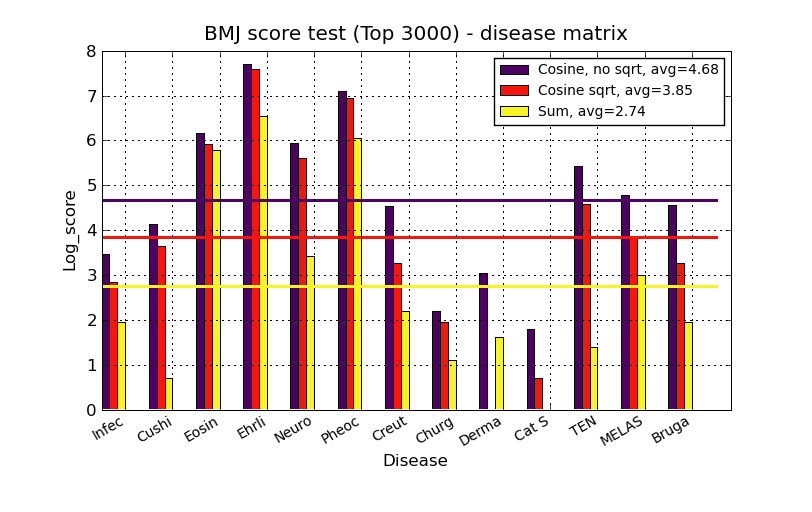
\includegraphics[width=0.9\textwidth]{barcharts/diseaseMatrix_bmj_hist_norm_3000_ns_cos_sqrt_cos_sum_nn.png}
        \end{center}
        \caption{Test of non-stemmed mean, median and max using normalization and cosine}
        \label{diseaseMatrix_bmj_hist_norm_3000_ns_cos_sqrt_cos_sum_nn}
\end{figure}
 
Cosine - Scores: [31,62,474,2220,377,1225,93,8,20,5,227,118,94] - In top 20: 2 \\
Cosine sqrt - Scores: [16,37,375,2001,270,1037,25,6, 0,1, 97, 45,25] - In top 20: 4 \\
Sum - Scores: [ 6,1,323, 691,30,427,8,2,4,0,3,19,6] - In top 20: 9 \\

\begin{figure}[h!]
        \begin{center}
          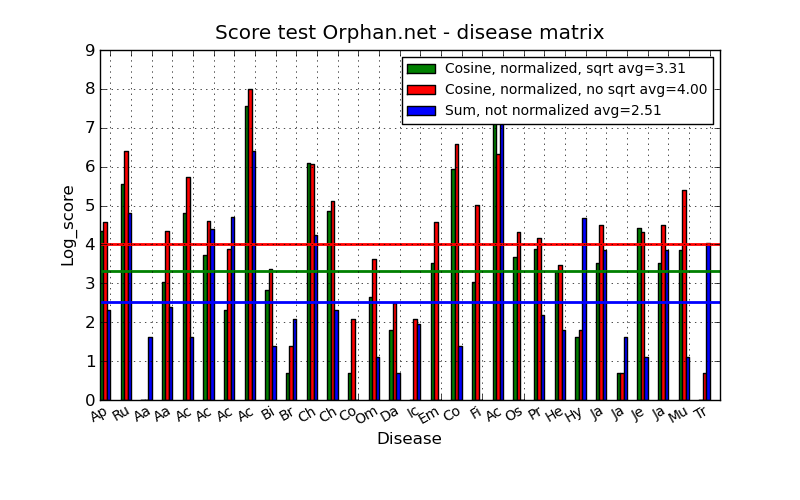
\includegraphics[width=0.9\textwidth]{barcharts/diseaseMatrix_orphan_hist_NOTnorm_3000_ns_cos_sqrt_cos_sum_nn.png}
        \end{center}
        \caption{Test of non-stemmed mean, median and max using normalization and cosine}
        \label{diseaseMatrix_orphan_hist_NOTnorm_3000_ns_cos_sqrt_cos_sum_nn}
\end{figure}
 
Cosine - Scores:[95,599,0,76,307,99,47,2989,28,3,430,165,7,37,11,7,97,717,150, 562,74,64,31,5,89,1,75,89,222,1] - In top 20: 8 \\
Cosine sqrt - Scores: [76,257,0,20,122,41, 9,1912,16,1,448,128,1,13, 5,0,33,380, 20,1687,39,47,26,4,33,1,83,33, 46,0] - In top 20: 11 \\
Sum - Scores: [9,123,4,10,4,81,109,601,3,7,68,9,0,2,1, 6,0,3,0,3000,0,8, 5,107,46,4,2,46,2,55] - In top 20: 20 \\

Stemmed:

\begin{figure}[h!]
        \begin{center}
          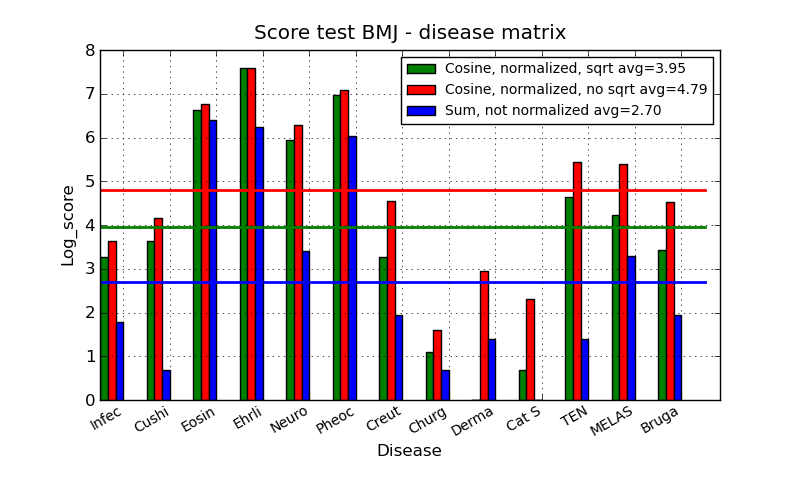
\includegraphics[width=0.9\textwidth]{barcharts/diseaseMatrix_bmj_hist_norm_3000_s_cos_sqrt_cos_sum_nn.png}
        \end{center}
        \caption{Test of non-stemmed mean, median and max using normalization and cosine}
        \label{diseaseMatrix_bmj_hist_norm_3000_s_cos_sqrt_cos_sum_nn}
\end{figure}

 
Cosine stemmed - Scores: [37,63,872,1963,533,1198,93,4,18,9,230,221,91] - In top 20: 3 \\
Cosine sqrt stemmed - Scores: [25,37,748,1970,384,1053,25,2, 0,1,102, 68,30] - In top 20: 3 \\
Sum stemmed - Scores: [5,1,597,511,29,413,6,1,3,0,3,26,6] - In top 20: 8 \\

\begin{figure}[h!]
        \begin{center}
          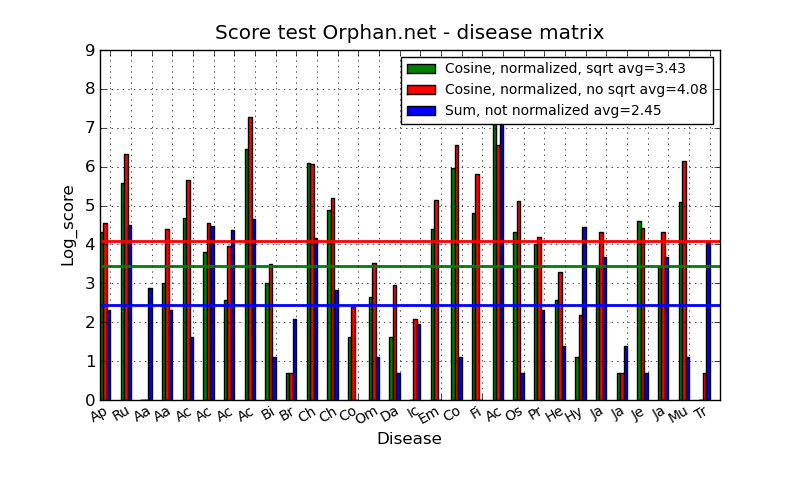
\includegraphics[width=0.9\textwidth]{barcharts/diseaseMatrix_orphan_hist_NOTnorm_3000_s_cos_sqrt_cos_sum_nn.png}
        \end{center}
        \caption{Test of non-stemmed mean, median and max using normalization and cosine}
        \label{diseaseMatrix_orphan_hist_NOTnorm_3000_s_cos_sqrt_cos_sum_nn}
\end{figure}

 
Cosine stemmed - Scores: [94,553,0,80,284,94,51,1454,32,1,433,181,10,33,18,7,169,710,334, 704,167,65,26,8,74,1,83,74,468,1] - In top 20: 8 \\
Cosine sqrt stemmed - Scores: [74,263,0,19,106,44,12, 635,19,1,446,133, 4,13, 4,0, 80,391,122,2137, 74,54,12,2,30,1,99,30,162,0] - In top 20: 13 \\
Sum stemmed - Scores: [9,90,17, 9,4,86,79,105,2,7,64,16,0,2,1, 6,0,2,0,3000,1,9,3, 84,39,3,1,39,2,59] - In top 20: 20 \\

When it comes to scoring diseases on in the disease matrix, the sum measure greatly outrival the cosine measure, with or without the square root transformation. If we look at the average values of the returned results, it seems that the stemmed version of the disease matrix is the best choice for optimized performance. \\

For the final test of measure and model, we compare the top results of the two matrices - term document and disease matrix. We will compare the different scores from the stemmed version of both matrix types since this seems to provide the overall best performance. In the figures \ref{termDoc_bmj_hist_3000_sum_dm_mea_cos_sqrt_td_max_cos_sqrt_td_mea_sum_td} and \ref{termDoc_orphan_hist_3000_sum_dm_mea_cos_sqrt_td_max_cos_sqrt_td_mea_sum_nn_td} below are bar chart of the best scores found for the prototype system:

\begin{figure}[h!]
        \begin{center}
          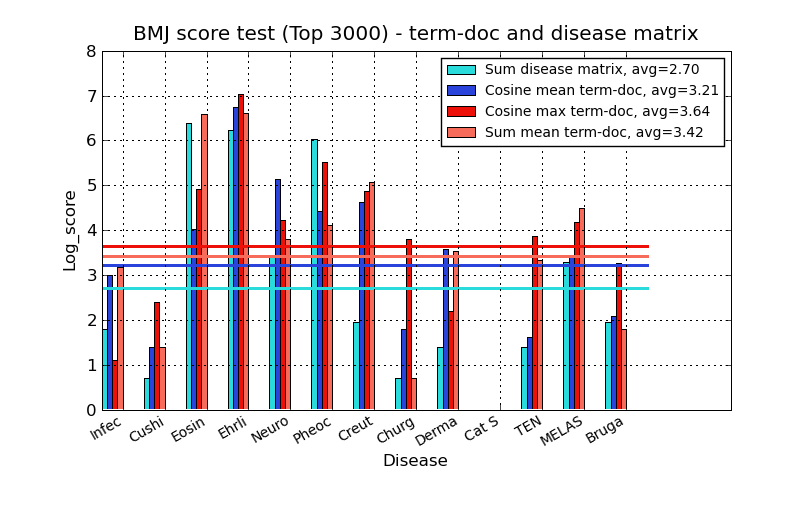
\includegraphics[width=0.9\textwidth]{barcharts/termDoc_bmj_hist_3000_sum_dm_mea_cos_sqrt_td_max_cos_sqrt_td_mea_sum_td.png}
        \end{center}
        \caption{Test of non-stemmed mean, median and max using normalization and cosine}
        \label{termDoc_bmj_hist_3000_sum_dm_mea_cos_sqrt_td_max_cos_sqrt_td_mea_sum_td}
\end{figure}
 
Sum: disease matrix - Scores: [ 6,1,323, 691,30,427,8,2,4,0,3,19,6] - In top 20: 9 \\
Cosine: mean stemmed sqrt - Scores: [19,3,22,1268,115,105,108,5,54,0,2,41,7] - In top 20: 6 \\
Cosine: max stemmed - Scores: [2, 10, 136, 1123, 68, 249, 130, 44, 8, 0, 47, 65, 25] - in top 20: 4 \\
Sum: term-doc mean - Scores: [23, 3, 720, 746, 44, 60, 158, 1, 33, 0, 27, 88, 5] - In top 20: 4 \\

\begin{figure}[h!]
        \begin{center}
          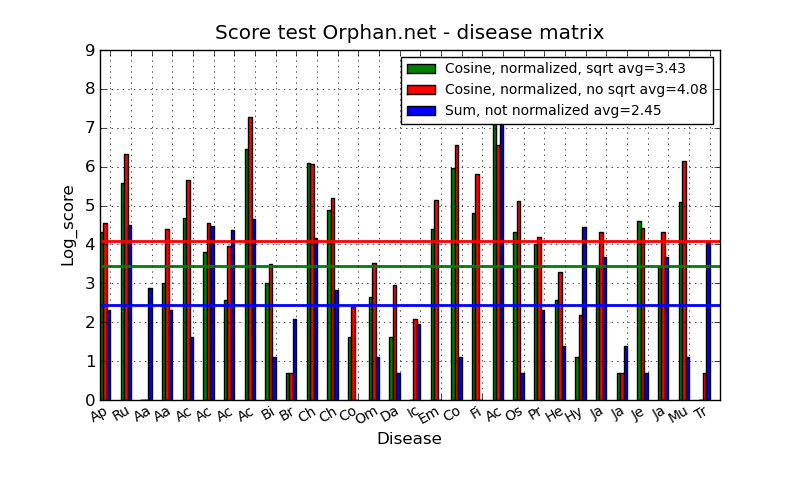
\includegraphics[width=0.9\textwidth]{barcharts/diseaseMatrix_orphan_hist_NOTnorm_3000_s_cos_sqrt_cos_sum_nn.png}
        \end{center}
        \caption{Test of non-stemmed mean, median and max using normalization and cosine}
        \label{termDoc_orphan_hist_3000_sum_dm_mea_cos_sqrt_td_max_cos_sqrt_td_mea_sum_nn_td}
\end{figure}

Sum: disease matrix - Scores: [9,90,17, 9,4,86,79,105,2,7,64,16,0,2,1, 6,0,2,0,3000,1,9,3, 84,39,3,1,39,2,59] - In top 20: 20 \\
Cosine: term-doc mean-sqrt - Scores: [4, 725, 75, 37, 38, 85, 68, 1651, 1, 23, 80, 15, 0, 26, 2, 218, 3, 13, 2, 3000, 1, 9, 14, 78, 84, 48, 3, 84, 1, 62] - In top 20: 13 \\
Cosine: term-doc max-sqrt - Scores: [12, 145, 0, 0, 93, 6, 2, 1842, 6, 25, 44, 15, 0, 15, 1, 0, 10, 0, 3, 3000, 7, 46, 4, 128, 115, 1, 24, 115, 2, 1] - In top 20: 19 \\
Sum: term-doc mean - Scores: [6, 708, 644, 28, 97, 460, 170, 2522, 1, 30, 190, 58, 0, 43, 6, 136, 3, 39, 16, 2636, 0, 8, 50, 33, 115, 53, 31, 115, 121, 124] - In top 20: 8 \\

Not only having the best average but also the right disease 9 out 13 (BMJ) and 20 out of 30 (Oprha.net) in the top 20 out of over 3000 diseases returned from a top 3000 document scores, using the simple sum similarity measure on a disease matrix seems to give both best recall and precision. This result is very interesting since the document-summed disease matrix was originally made as model for fast tests before implementation in the large term document matrix. This could imply that a summation of the document vectors for each individual disease seems to enchance the values of information carrying terms with the TF-IDF taking care of too common and non-information containing terms. The summation also efficiently eliminates the problem of noisy overview articles \ref{Overview}. \\

One of the noteworthy things that can be learned from the bar charts made in this and the two previous sections is that there should be a lower bound on the number of documents per disease. Acropectorovertebral dysplasia is a premium example that the system needs to have a lower bound on the number of medline records that are gathered for each disease. This is in order to ensure that the system will be able make a reasonable qualified guess on the disease.

\subsection{Clustering of the results}
\fxnote{Needs to be refined}
Currently we are only able to make clusters from disease matrices, we have chosen to make a cluster of the top 20 diseases return to see how these lie in relation to each other. Of special interest is Cat scratch disease which our system almost always lists correctlu. %See dendrogram \ref{Dendro_cat_scratch_disease}, it can be seen how ...

%% \begin{figure}[h!]
%%         \begin{center}
%%           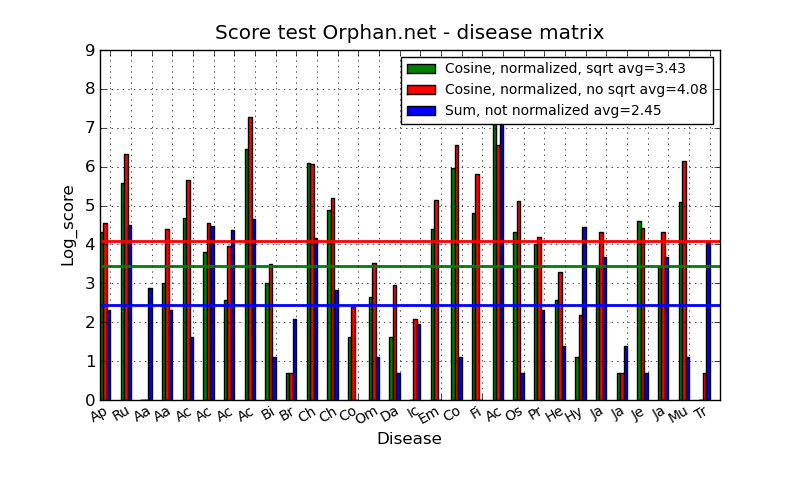
\includegraphics[width=0.9\textwidth]{barcharts/diseaseMatrix_orphan_hist_NOTnorm_3000_s_cos_sqrt_cos_sum_nn.png}
%%         \end{center}
%%         \caption{Test of non-stemmed mean, median and max using normalization and cosine}
%%         \label{Dendro_cat_scratch_disease}
%% \end{figure}


%% \subsection{The reduced semantic space and keyword extraction}

To be written...




\subsection{On overview article noise and concensus normalization\label{Overview}}

Overview articles
Unfortunately there is overview articles that can pollute the search results and if overview articles are found in many of the top scoring diseases, it could present a problem. When we run the concensus method as described in the \ref{CosineScore}, an overview article would potentially get an unfair high score since it gets summed up to 240 times. Though overview articles represents an element of noise, the normalization of the vectors in the vector space model should in theory down weight the highly summed documents. We also tested to the most common overview article (240 occurrences), to see if it could be a problem, using the Orpha.net disease cases among top 3000 (documents). The overview article was present in less than 1 out of 8 searches which is not a significant amount. The disease matrix on the other hand is less prone to the same problem, as it summarizes all information about a disease into one vector. \\

Concensus normalization
During a point in the testing of the term document matrices, we got the idea to try and divide each label with the number of documents it had been summed over. This could in theory normalize the label in the top score of returned results, as labels being over-represented in e.g. the bottom of the top score list would be weighted down. However, as this might be a good theoretical idea, it did not quite amount ot anything useful. The results for running this on the stemmed term document matrix, using the cosine measures, is: \\

Mean: [99, 210, 804, 1216, 507, 667, 167, 309, 502, 50, 330, 695, 424] \\
Median: [1036, 989, 1432, 948, 668, 1301, 1315, 1687, 1429, 1233, 1696, 1494, 1322] \\
Max: [1034, 989, 1447, 1084, 635, 1284, 1293, 1687, 1414, 1233, 1696, 1491, 1321] \\

It does not take a bar chart to see that these values are pretty off the top 20. The idea might be good enough but it would have to be on a different model or data set than the one we use.


\chapter{Conclusion\label{Conclusion}}


\chapter{Future Works\label{FutureWorks}}


\bibliographystyle{unsrt} % nat
\bibliography{referencelist}
%% 
\addcontentsline{toc}{section}{Reference list}

\appendix
\chapter{Source Code}

This is our source code and a plain text file containing all our test
results written as python lists. The source code is arranged the way
the system data flow is structured. The source code is also available
at
\href{git://github.com/hmbachelor/bachelor.git}{git://github.com/hmbachelor/bachelor.git}.
But be warned, some of it is a mess. There is a lot of junk code,
redundant code. It needs a spring cleaning, but that will have to
wait.

\subsection*{Disease Crawler}
\lstinputlisting{../PubMedParser/src/DiseaseCrawler.py}

\subsection*{PubmedSIR}
\lstinputlisting{../PubMedParser/src/PubmedSIR.py}

\subsection*{TermDoc}
\lstinputlisting{../PubMedParser/src/TermDoc.py}

\subsection*{DiseaseMatrix}
\lstinputlisting{../PubMedParser/src/DiseaseMatrix.py}

\subsection*{SearchTermDoc}
\lstinputlisting{../PubMedParser/src/SearchTermDoc.py}

\subsection*{Cluster}
\lstinputlisting{../PubMedParser/src/Cluster.py}

\subsection*{DistanceMeasures}
\subsubsection{CosineMeasure}
\lstinputlisting{../PubMedParser/src/CosineMeasure.py}
\subsubsection{SumMeasure}
\lstinputlisting{../PubMedParser/src/SumMeasure.py}

\subsection*{SearchCases}
\lstinputlisting{../PubMedParser/src/SearchCases.py}

\subsection*{Interfaces}
\subsubsection{FilterInterface}
\lstinputlisting{../PubMedParser/src/FilterInterface.py}
\subsubsection{SearchInterface}
\lstinputlisting{../PubMedParser/src/SearchInterface.py}

\subsection*{Auxilary modules}
\subsubsection{IOmodule}
\lstinputlisting{../PubMedParser/src/IOmodule.py}
\subsubsection{TextCleaner}
\lstinputlisting{../PubMedParser/src/TextCleaner.py}
\subsubsection{RecordHanlder}
\lstinputlisting{../PubMedParser/src/RecordHandler.py}
\subsubsection{Stemmer}
\lstinputlisting{../PubMedParser/src/Stemmer.py}
\subsubsection{StopwordRemover}
\lstinputlisting{../PubMedParser/src/StopwordRemover.py}
\subsubsection{Stat}
\lstinputlisting{../PubMedParser/src/Stat.py}
\subsubsection{SearchTermCombiner}
\lstinputlisting{../PubMedParser/src/SearchTermCombiner.py}

\chapter{Raw test data}

The raw test data are available in the github repository in the file
called testModule.py. This file needs some serious cleaning.



\end{document} 
